%Elsevier-specific stuff
%\documentclass[review]{elsarticle}
\documentclass[5p]{elsarticle}
\usepackage{lineno,hyperref}
\usepackage{tabularx}
\modulolinenumbers[5]
%\bibliographystyle{elsarticle-num}
\bibliographystyle{model2-names.bst}
\biboptions{authoryear}

%Other packages and general latex fields.
\usepackage{url}
\usepackage{color}
\usepackage{graphicx}
\usepackage{epstopdf}

\usepackage{caption}

%%%%%%%%%%%%%%%%%%%%%%%%%%%%%%%%%%%%%%%%%%
\begin{document}
\begin{frontmatter}
\title{gPhoton: A Time-Tagged Database of GALEX Photon Events}

% Authors section.
\author[millionconcepts]{Chase Million\corref{chasecorref}}
\cortext[chasecorref]{Corresponding author}

\author[stsci,csc]{Scott W. Fleming}
\author[stsci]{Bernie Shiao}
\author[carnegie]{Mark Seibert}
\author[ucolorado]{Parke Loyd}
\author[appstate]{Michael Tucker}
\author[stsci]{Myron Smith\fnref{myronnewaddress}}
\author[stsci,csc]{Randy Thompson}
\author[stsci]{Richard L. White}
\author[stsci,csc]{Karen Levay}

% Addresses section.
\address[millionconcepts]{Million Concepts LLC, 2204 Mountain View Ave., State College, PA 16801, USA}
\address[stsci]{Space Telescope Science Institute, 3700 San Martin Dr, Baltimore, MD 21218, USA}
\address[csc]{Computer Sciences Corporation, 3700 San Martin Dr, Baltimore, MD 21218, USA}
\address[carnegie]{The Observatories of the Carnegie Institution of Washington, 813 Santa Barbara Street, Pasadena, CA 91101, USA}
\address[ucolorado]{Department of Astrophysics and Planetary Science, University of Colorado, Boulder CO}
\address[appstate]{Dept. of Physics and Astronomy, Appalachian State University, Boone, NC 28608, USA}
\fntext[myronnewaddress]{Current Address: National Optical Astronomy Observatory, 950 N. Cherry Ave., Tucson, AZ 85719}

% Since \fnref{} in the author page already defines a footnote with a '1' mark, increment the footnote counter now.
\addtocounter{footnote}{1}

\begin{abstract}
gPhoton\footnote{\url{https://github.com/cmillion/gPhoton}} is a new database product and software package that enables analysis of GALEX ultraviolet data at the photon event level. The project's standalone, pure-Python calibration pipeline reproduces functionality of the original mission pipeline to reduce raw spacecraft data to lists of time-tagged, sky-projected photon events which are then hosted in a publicly available database by the Mikulski Archive at Space Telescope (MAST). This database contains approximately 130 terabytes of data describing approximately 1.1 trillion sky-projected GALEX photon events. A small suite of addtional command line tools establish a front end with which users can generate calibrated light curves and images from the photon-level data at user-defined temporal and spatial scales. The gPhoton software and source code are publicly available under a permissive license and will continue to be developed and maintained in the future. We describe the motivation, design, and implementation of the calibration pipeline, database, and tools, with emphasize on divergence from prior work as well as challenges created by the large data volume. We summarize the astrometric and photometric performance of gPhoton output as compared to the original mission pipeline and using the LDS749B and LB227 white dwarf standard stars. As an example of short time domain science capabilities, we describe new flare observations of the known M dwarf flare star CR Draconis.
\end{abstract}

\end{frontmatter}

\linenumbers

\section{Introduction}
\subsection{GALEX Overview}
The Galaxy Evolution Explorer \citep{mar2005} was a NASA Small Explorer (SMEX) telescope that surveyed the sky in the ultraviolet over ten years between launch on 28 April 2003 and spacecraft termination on 28 June 2013. The spacecraft, instruments, data and calibration are well described in previous publications \citep{mor2005,mor2007} and the mission'��s technical documentation\footnote{\url{http://www.galex.caltech.edu/wiki/Public:Documentation}}. We will restrict discussion to topics that have not appeared elsewhere in the literature, are of particular importance to the gPhoton project, or are otherwise necessary for completeness.

GALEX carried two microchannel plate detectors (MCP), simultaneously exposed via a dichroic, and had a 1.25 degree field-of-view (FoV). It observed in two broad ultraviolet (UV) bands centered around $1528\,\rm{\AA}$ (Far Ultraviolet or ``FUV'') and $2271\,\rm{\AA}$ (Near Ultraviolet or ``NUV'').  The FUV detector failed in May of 2009, but the NUV detector continued to operate until the end of the mission. The detectors could observe in either direct imaging or slitless spectroscopic (grism) modes. Observations were conducted while the spacecraft was on the night side of each orbit (an ``eclipse''), which lasted 1500-1800 seconds. To avoid detector burn-in or local gain sag effects caused by depletion of electrons in the multiplier plate, and to smooth over local irregularities in detector response, the telescope did not stare at a fixed location on the sky during an observation, but continuously moved the boresight relative to the target position. Several boresight patterns, or ``modes,'' were used over the course of the mission, with consequences for the nature of the corresponding observations and data.

In the most basic ``dither'' mode, the spacecraft boresight would trace out a tight spiral pattern with a radius of $\sim 1'$. Dither mode was used most often for Deep or Medium Imaging Surveys (DIS, MIS) in which a full eclipse was spent observing a single region of the sky. In the All-sky Imaging Survey (AIS) mode, the spacecraft boresight would jump between multiple positions (or ``legs'') on the sky for short integrations of $\sim 100$ seconds each. Between each leg, the detector was set to a non-observing, low voltage state. This resulted in one independent observation (or ``visit'') per leg. A mode called ``petal pattern'' was used to distribute the flux from particularly bright targets across the detector. Petal pattern is in some ways sim similar to the AIS mode, but with the legs tightly clustered into the approximate area of a single FoV and with the detector remaining in its nominal high-voltage state in between.

On 4 May 2010, an event referred to by the mission team as the ``Course Sun Point'' (CSP) anomaly---referring to the safe mode entered by the spacecraft at that time---resulted in image degradation of the NUV detector. The CSP anomaly precipitated severe streaking in the detector's Y-direction, likely due to a failed capacitor. Although the effect was largely corrected through subsequent calibration and onboard adjustments\footnote{\url{http://www.galex.caltech.edu/wiki/Public:Documentation/Chapter_8}}, observations taken between 4 May and 23 June 2010 have substantially worse point spread functions, and caution should be exercised when comparing observations made before this time range to observations made after.

NASA support for the mission ended in February of 2011. At that time, ownership of the spacecraft was transferred to the California Institute of Technology for a phase called the ``Complete the All-sky UV Survey Extension'' (CAUSE), during which operating costs were solicited from individuals or institutions, and spacecraft engineering constraints related to field and source brightness were relaxed, making it possible to observe bright regions of the sky that were off limits during primary mission [CITE]. Spacecraft slew rate limits were also relaxed, permitting a high-coverage ``scan mode'' that swept across several degrees of sky in a single integration. Ownership of the CAUSE-phase data resides with each of the primary investigators, and only a small fraction of it has been made available to the public through MAST at the time of writing, although much of the raw data has been copied to MAST systems. Although the new calibration capabilities of gPhoton may be of particular value in using and interpreting CAUSE data generally and scan mode observations of very bright or dense fields in particular, this paper (and the current gPhoton database) only includes the direct imaging data through the end of the NASA-supported mission, corresponding to General Release 7 (GR7) in the MAST archives. Future work may add gPhoton support for CAUSE phase, scan mode, or spectroscopic data collected throughout the mission. Through GR7, GALEX collected data over 34,389 (direct image) eclipses, which amount to $\sim 18$ TB of raw data and $\sim 14$ TB of reduced image data, covering 76.9\% of the sky in at least one band.

In Section \ref{motivation} we describe the motivation behind constructing the gPhoton database and software suite. In Section \ref{database} we describe the design and content of the $\sim 1.1$ trillion row database hosted at MAST. In Section \ref{softwaretools} we describe the primary modules to use for generating photon lists, light curves and images. In Section \ref{implementation} we discuss implementation challenges we encountered, and our solutions to those problems, some of which may be applicable to other large databases low level scientific data. In Section \ref{calibration} we present tests of the calibration precision by studying the astrometric, relative, and absolute fluxes produced by the software. Finally, in Section \ref{scienceexamples}, we highlight an example science case enabled by gPhoton: stellar flares from CR Draconis.

\section{Motivation}
\label{motivation}
Micro-channel plate (MCP) detectors like those on GALEX are non-integrating detectors---sometimes called ``photon-counting''---that can record position and time information individually for every incident photon (``event''). The GALEX detectors were capable of recording data with a time resolution of five microseconds, though the vast majority of observations were made in a compressed mode at five millisecond resolution. Due primarily to computer storage and processing constraints, calibrated GALEX data was only released and archived by the mission as either per-visit or multi-visit (coadded) image maps with exposure depths on the order of hundreds to thousands of seconds. Although the GALEX mission's data calibration pipeline (hereafter referred to as the ``mission pipeline'') was capable of producing aspect-corrected photon list files (called ``extended'' or ``x-files''), this was rarely done as part of instrument diagnostics or by special request of members of the scientific community, [CITE Welsh, what else?] and the team documented very little on the detector performance or calibration on timescales shorter than $\sim 100$ seconds.

Advances in storage and processing capabilities now make storage, distribution, and analysis of the photon-level data technologically feasible. By the end of the mission, however, the mission pipeline had grown to sufficient complexity and dependence on its software and hardware operating environment at Caltech that attempts to run it outside of that environment proved unsuccessful. We undertook the gPhoton project, in part, to migrate key functionality of the mission pipeline into a stand-alone, open source software base that is robust enough to operating environment to serve as a jumping off point for future researchers to modify or improve the calibration or otherwise build on the legacy of this unique data set. Another major objective was to enable the creation of calibrated light curves and images at user-specified spatial and temporal scales, permitting studies of short time-domain variability over a significant fraction of the sky in the UV for the first time. Our project design goals included the following key features:
\begin{itemize}
\item{Creation of a database, containing (nearly) all photon events from the mission, that can be queried efficiently.}
\item{Software that can perform the necessary calibrations (astrometric, photometric, exposure time, etc.), at quality comparable to the original mission pipeline, over visit- and coadd-level timescales.}
\item{Allow users to flexibly create images (as a coadds over one or more specified time ranges) or an image cubes (as sequences of such images).}
\item{Allow users to create light curves with a specified time intervals and bins depths.}
\item{Lower the barrier to entry of working with short time domain GALEX data by, e.g., minimizing the number of primary (forward-facing) modules most users will need, wrapping the SQL queries behind a python interface, creating commonly used output file formats like FITS and comma separated values (CSV), etc.}
\end{itemize}

While the gPhoton project does reproduce much of the core functionality of the mission pipeline, it is not intended as either a full migration or a faithful port of the original mission pipeline. As will be described, some archived output files from the mission pipeline are used where deemed expedient, and the calibration and reduction methodology has been modified in some places in service to both computational efficiency and the unique properties and uses of photon-level data.

\section{Description of the Database}
\label{database}
\subsection{Description of Data Products from the Mission Pipeline Used By gPhoton}
During the GALEX mission, data were downlinked from the spacecraft and assembled on the ground into monolithic telemetry files (-tlm). The ingest stage of the mission pipeline split these into various types of encoded raw detector event and spacecraft state (-scst) data, which included coarse aspect solutions from the onboard star tracker at one-second resolution, as well as spacecraft housekeeping records. The most important class of encoded raw detector data for gPhoton, containing nominal scientific observations, were the -raw6 files. The -raw6 were decoded with a sequence of bitwise manipulations into lists of raw detector positions ($x$ and $y$) with timestamps for all detector events. These raw positions were further adjusted with ``static'' (detector-space) calibrations for wiggle, walk, nonlinearity and distortion, described more completely in \citet{mor2007}. For post-CSP data (after eclipse number 37460), the calibration was modified to correct and account for changes to the detector behavior and parameters in the onboard software. The most substantial of the post-CSP calibration changes was the addition of a processing step to correct for detector streaking caused by the anomaly and correlated strongly to the “YA” value of the raw position data (one of many intermediate raw data values used in derivation of detector event positions).

\subsection{Construction of the Database}
The database is populated using photon list files produced by running event extraction on the full corpus of data, up to and including GR7.  The first step in generating the database was to create aspect-corrected photon events as CSV files.  Starting with the raw photon event (-raw6), refined spacecraft attitude (-asprta), and spacecraft state (-scst) files available at MAST, the celestial coordinates of the photon events are calculated and then exported to the CSV file. At this stage, the CSV file contains the time of the photon event, the event positions on the detector, the aspect-corrected positions on the sky (as RA and DEC), and status flags used to track a variety of conditions related to the detector readout. The vast majority of users will only be interested in photon events for which the photon file flag value is equal to 1, indicating nominally processed data.

Only a subset of the photon events from a given eclipse are able to have aspect-corrected positions calculated (most often because only a subset of photon events in an eclipse correspond to an observation, others happen during dead time, slewing, etc.  Therefore, a total of four CSV files are created: two CSV files for FUV and NUV data that contain aspect-corrected photon events, and two CSV files for FUV and NUV data containing photon events that were not aspect-corrected. The non-aspect-corrected photon events are still loaded into a database, because they are used for estimating dead time corrections (see Section \ref{deadtimedesc} for details). When events cannot be aspect-corrected, their right ascension and declination values are assigned values of \emph{NULL} in the photon list file. The distinction between this ``null data'' and nominal or ``non-null data'' is important, as it is treated differently in both the database and high level calibration.

A large fraction of data are not aspect-correctable because they fall in time ranges that are not covered by the refined aspect solutions. Such gaps occur when the detector voltage is ramping up or down between observations or when the slew rate was too high (as between legs of a petal pattern observation) or the stellar field too sparse for the aspect refinement pipeline to obtain a solution. Null events can also arise from cases where events fall outside of the main detector FoV, including data arising from the stims, detector noise, or downlink errors. At present, data that fall within regions of the detector are also not aspect corrected. Many GALEX hotspots are known to be transient, however, such that the masks can block valid observational data; any version of the pipeline and database will aspect-correct the masked data and apply the mask in the client side at the same time as response correction, at discretion of the user.

For performance optimization purposes, the event-level data is distributed over multiple databases. The non-null (aspect corrected) data are spread across ten different databases organized by celestial declination, with bounding ranges selected to approximately balance the number of rows per database.  The ten database tables are further divided into a total of 999 partitions. Each partition is then further divided into ``zones'' of $30''$. We make use of the fast zone matching algorithm described in \citet{gra2006} for loading and querying the database.  Both the database boundaries and the number of $30''$ zones assigned to each partition were defined so that the databases are of similar sizes.  This was accomplished by assuming the total number of photon events in a given eclipse is distributed evenly across that eclipse's footprint.  Then, the cross-section of that eclipse's footprint against the zone boundaries is calculated to determine which zones that eclipse overlaps.  The number of photons in each zone from this eclipse is estimated based on the cross-sectional area, e.g., if a given eclipse spans two zones, but only 10\% of the eclipse's footprint is in one of the zones, 90\% of its total photon events would be considered to belong to the first zone, and 10\% to the other.

This method of estimating photon events in each zone is not precise, since it assumes photon events are evenly distributed across the eclipse, but it does serve as a quick approximation to define the database boundaries and partition assignments by not requiring to actually compute the zone membership for all 1.1 trillion photon events beforehand.  The distribution of the ten databases on the sky is shown in Fig.\ \ref{dbdist}, along with a table summarizing the declination ranges and number of photon events in each database (Table \ref{dbcounts}). The assignment to a database or partition is strict, leaving open the possibility that a user's query spans two databases. The majority of normal queries access only a single database, but queries that do span multiple databases are handled on the server, transparent to both the software and end users. Null data which were not aspect corrected reside in a single database.  {\color{red}How are the non-null and null tables indexed (which columns)?}

\begin{figure}
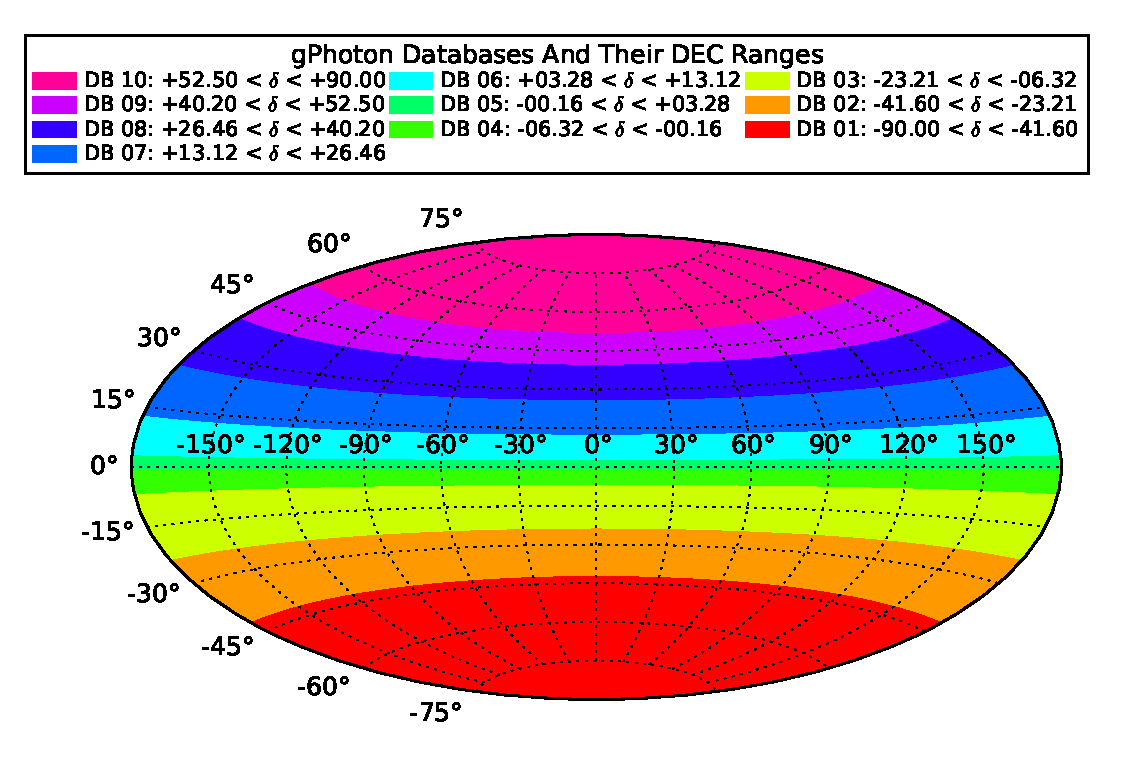
\includegraphics[scale=0.48]{FigDBDist.eps}
\caption{The DEC boundaries of the ten individual databases holding the full corpus of photon data. There are a total of 999 partitions across the ten databases, each with a variable number of $30''$ zones (stripes of DEC).  The number of zones in each partition, and the number of partitions in each database, were assigned so that the size of the ten databases would be roughly equal to each other. \label{dbdist}}
\end{figure}

\begin{table}
\caption{Non-Null Photon Events Per Database\label{dbcounts}}
\begin{tabularx}{.47\textwidth}{lllXX}
\hline\hline
DB & min $\delta$ & max $\delta$ & N\_FUV & N\_NUV\\
   & deg          & deg          & x$10^9$ & x$10^9$\\
\hline
1 & -90.00 & -41.60 &   6.257390699 &  86.634587040\\
2 & -41.60 & -23.21 &   6.381213422 &  86.548536265\\
3 & -23.21 &  -6.32 &   6.581269082 &  86.661438444\\
4 &  -6.32 &  -0.16 &   5.855815141 &  86.824342990\\
5 &  -0.16 &   3.28 &   5.918115466 &  87.675967291\\
6 &   3.28 &  13.12 &   6.431868719 &  86.895361749\\
7 &  13.12 &  26.46 &   6.230197521 &  87.197846131\\
8 &  26.46 &  40.20 &   5.392882518 &  86.855190790\\
9 &  40.20 &  52.50 &   5.394019934 &  86.683794328\\
10 &  52.50 &  90.00 &   6.540819967 & 100.482179843\\
\hline
\end{tabularx}
\end{table}

\section{Description of the Software Tools}
\label{softwaretools}
There are four primary modules included in gPhoton and described in Table \ref{moduledesc}. These utilities are all written in Python and released under a permissive license. With the exception of gPhotonPipe, the tools can be called either from the command line or imported as Python modules. When imported as modules, output is returned in a Python data structure. The command line utilities draw upon a large a large number of supporting functions which will not be described in this paper but are possibly of interest to users who want to perform advanced or specialized analyses with the gPhoton data or even modify the functionality to fit their individual needs. For more information, users are encouraged to consult the documentation available in the software repository, or at the MAST page for the project: \url{https://archive.stsci.edu/prepds/gphoton/}.

While the tools have individual syntaxes to fit their specific functions, a few conventions are standard across all of them. Sky positions are reported as a two-element vectors (right ascension and declination) in J2000 decimal degrees. Time ranges (or ``bins'') are defined as two-element vectors where the first element is the start time and the second element is the end time. The gPhoton project defines timestamps in units of ``GALEX time'' throughout, where $t_{\rm{GALEX}} = t_{\rm{UNIX}} - 315964800$ seconds. To avoid double counting of boundaries, both spatial and temporal ranges are generally taken to be inclusive of the lower value and exclusive of the higher value.

By default, the database tools define an effective detector FoV 1.1 degrees in diameter. This is to conservatively trim data observed on the edges of the GALEX MCPs, which suffer from poorly understood sensitivity and spatial distortion. Data near the edges may be useful to cautious and knowledgeable investigators, though, so the effective detector size is adjustable from the command line. This conservative trimming of the physical FoV does not eliminate problems caused apertures, annuli, or images overlap, and are therefore clipped by, the boundary of the \emph{effective} FoV. For meaningful photometry, sources must be clear of both the physical and effective FoV boundaries.

\begin{table}
\begin{tabular}{|p{2cm}|p{6cm}|}
\hline
	{\bf Module} & {\bf Function}\\\hline
	gPhotonPipe & Generates aspect-corrected photon lists from a small set of user supplied input files.  The input files are normally archived products from the original mission pipeline. Output from gPhotonPipe was used to populate the photon event database that the other modules query and, therefore, the majority of researchers will not need this module.\\\hline
	gFind & Provides information on the available raw exposure depths and time ranges for any location on the sky.\\\hline
	gAperture & Generates a light curve (returned as a table of times, calibrated fluxes, and additional parameters) for a given coordinate, time sampling, and aperture size.\\\hline
	gMap & Creates an image (in units of counts and/or calibrated fluxes) and/or image cubes (also in units of counts and/or calibrated fluxes), for a given area of the sky and (optionally) time sampling.\\
\hline
\end{tabular}
\caption{Summary of Primary gPhoton Modules}
\label{moduledesc}
\end{table}

\subsection{gPhotonPipe}
The gPhotonPipe calibration implements a subset of the steps from the original mission pipeline in order to perform detector-level calibration and aspect correction of photon events. The module accepts the raw scientific data file (-raw6), the spacecraft state file (-scst), and one or more refined aspect solution files (-asprta). It returns a ``photon list file'' in CSV format, where each row corresponds to a detector event and records information such as the raw and calibrated detector event positions, sky projected (de-dithered) event positions, and a flag that encodes metadata on the photon event, propagating flags from the aspect solution files and also encoding whether the event falls in a known detector hotspot region. Please see the project documentation for a description of these columns. A flag value of zero indicates that there were no problems with the calibration of an individual event, and this is generally the metric used to determine which should be used by the other tools for later analysis. The photon list files produced by gPhotonPipe are analogous (but not identical) to the extended photon list (-x) files that were occasionally produced (but not archived) by the mission.

Note that all the inputs to the stand-alone calibration pipeline (-raw6, -scst, and -asprta files) are products from the original mission pipeline that are archived at MAST.  By using these archived mission products directly, gPhoton avoids the need to recreate either the ingest or aspect correction stages of the mission pipeline. If an aspect file is not supplied, then gPhotonPipe will attempt to query the MAST database of -asprta data.  Manually specifying the aspect file is possible for researchers who wish to further refine or modify the mission-provided aspect solutions.

\subsection{gFind}
This gFind module allows the user to query the available exposure depth of a particular target. Given a target position, gFind returns the estimated (raw) exposure depth of available data over the whole mission, separated into time ranges corresponding roughly to discrete observations of the target. Rather than using the visit-based bookkeeping of the mission, which distinguished between observation modes and survey type, gFind uses the photon events themselves. A given position on the sky is considered to be observed if valid data exists in a time range where the position falls within one effective FoV radius of the spacecraft boresight, as defined by the mission-provided refined aspect solution (-asprta). Distinct time ranges are identified based on a user-adjustable parameters that define the maximum allowable gap between two events for those data to be considered contiguous (or, in other words, part of the same observation) and the minimum raw exposure depth required for an observation to be considered valid.

\subsection{gAperture}
This module extracts and calibrates event-level data from the database to produce light curves, given user-specified parameters that can include target position, photometric aperture, background annuli sizes, desired integration depth (i.e., bin size), and time range or ranges. Rather than performing photometric measurements on pixelized and integrated images, as the mission pipeline did, gAperture performs aperture photometry by means of cone searches on the sky positions of individual photon events, enabling analysis at the native spatial resolution of the data. Each photon event is weighted by the detector flat value at the spot on the detector on which it occurred, using the mission-produced flats. All events within a given time bin are then weighted by the effective exposure time for the whole detector over that time range. Output from gAperture, which include a very large number of parameters related to the photometric reduction, can be written to CSV-format tables for later analysis. Of note are columns corresponding to bin ranges, effective exposure time, intermediate values such as total number of events within the aperture, calibrated source brightness in counts, physical flux, and AB magnitude units derived with a number of background estimation methods (see below), measurement error, and warning flags coding for a number of conditions that may bias photometric results. Please see the project documentation for a description of gAperture data columns.

\subsection{gMap}
This module creates integrated images and/or image cubes for targeted regions of the sky and specific time ranges, up to and including full depth coadds. Users can request either ``count'' images, which have not been corrected for exposure time or response (often useful for astrometry, diagnostics, or quick-looks), or ``intensity'' images, which are fully calibrated and suitable for photometric analysis. The images produced by gMap are analogous to the imaging data products produced by the mission pipeline, but with additional flexibility via user-tweakable parameters (e.g. dimensions, depth, edge trimming). If given a sequence of time ranges or a bin size, gMap will also produce ``count'' and/or ``intensity'' image cubes, which, at full resolution, were never available from the mission pipeline. All images are written in the Flexible Image Transport System (FITS) format that include headers populated using the World Coordinate System (WCS) standard.  As with relative response correction in gAperture, rather than generating a relative response map, the individual events are simply weighted by the flat value assigned to the detector regions on which they fell. In the current release, the exposure depth at the center of field is applied evenly across the whole image. This is not a good approximation in a large number of cases, particularly when the diameter of the image is not a small fraction of the diameter of the detector FOV; a spatially aware exposure time correction is planned for a future software build.

\section{Implementation Challenges and Solutions}
\label{implementation}
Numerous challenges have arisen during the development of this project, and our solutions to some of these may be helpful to other MCP or photon-level data investigations. The details may also be of general interest to users of our software suite.  We elaborate on several of these key components related to calibration and processing of the gPhoton data, noting that as the software is continually improved, some of these aspects may change.  Whenever conflicting information exists, the documentation in the repository takes precedence.

\subsection{Exposure Dead Time}
\label{deadtimedesc}
Microchannel plates are subject to a global exposure ``dead time'' effect caused by the inability of the detector to process more than one event at a time. The effect therefore scales as a function of total global detector count rates: as count rates go up, the fraction of exposure lost to dead time likewise increases, and is linear up to approximately 109 counts per second (cps) in FUV and 311 cps in NUV (demarcating a 10\% rolloff in response) \citet{mor2007}. Other MCP instruments have used this global count rate relationship as a means to estimate the dead time correction factor. The GALEX detectors, however, were equipped with four built-in electrical pulsers (``stims'') located off the main detection window that produced a known rate of events (between all four, 79 cps). The mission pipeline extracted these stim events as a direct proxy for the exposure dead time effect. That is, the ratio of the measured stim count rate to the canonical stim count rate is equivalent to the ratio of the effective exposure time to the commanded exposure time. However, one must also consider the contribution of counting statistics in this estimate.

The shortest standard GALEX integrations on single targets were the $\sim 100$ second observations in the AIS survey. Assuming zero dead time, the 1-sigma error in the stim rate due simply to Gaussian counting statistics would be around 0.9 counts per second (cps) or $\sim 1$\%. This level of error is negligible as compared to other sources, and, indeed, was not even propagated by the mission pipeline. For shorter integrations, however, like those that can be produced by gPhoton, the errors in the exposure time produced by estimating dead time from stims become quite meaningful. For a ten second and one second observation, respectively, with zero dead time, the 1-sigma errors are $\pm 2.81$ cps ($\sim 2.5$\%) and $\pm 8.9$ cps ($\sim 10.1$\%). The problem compounds for real observations, during which the fractional dead time can range from 10\% to 30\%, which for a 10-second integration, produces 1-sigma errors of $\sim 3.8$\% and $\sim 4.3$\%, respectively.

The solution used by gPhoton is to use the linear relationship between global count rate and dead time, which holds for reasonably low global count rates, to produce an empirical exposure time correction as a function of global count rate. GALEX has typical global count rates of 10,000 cps or more, making the 1-sigma error due to counting statistics truly negligible even for short integrations. The mission team did produce such an empirical dead time formula early on, but it suffered from a few problems that required us to revisit the problem and produce our own analysis. For one, while the result was recorded, the actual methodology was not, making it impossible to reproduce. Also, because it was early in the mission, extremely high count rate fields (in the non-linear response regime) of the detector had not been observed and were therefore not included in the analysis. Finally, the original analysis produced only a single model that, because their behavior was deemed so similar, simultaneously covered both the FUV and NUV detectors.

We plot global detector count rates against stim count rates. {\color{red}[Include this plot with best-fit slopes for both bands!]} We used exposure times that had been corrected for shutter (see Section \ref{effexptime}), but not dead time, when calculating these rates. In this analysis, we assume the foreground signal follows a linear model with two parameters (slope and intercept), and Gaussian counting errors in both $x$ and $y$. For the background, we also used a linear model with unknown parameters. This ``mixture model'' was sampled by Markov Chain Monte Carlo (MCMC) against the data for $\sim 1000$ observations in each band to produce maximum likelihood model parameters for the stim count rate as a function of global count rate in both bands, which could then be converted to a fractional dead time by comparing the stim count rate against the reference rate. Rather than directly adopting the quoted stim reference rate of 79 cps for both bands, we used the maximum likely y-intercept value as the reference rate. This produced models that differed in each band by about 3\%, which can be significant for GALEX. Thus, gPhoton treats the dead time correction slightly differently than the mission pipeline.

\subsection{Effective Exposure Time}
\label{effexptime}
The effective exposure time is computed as the raw exposure time (the difference between the observation start and end time), minus the amount of time considered ``shuttered,'' then scaled by the global dead time.  {\color{red}Add equation here.} Shuttered periods are those periods of significant length, for our purposes, considered to be 0.05 seconds or more, during which no valid observational data is available. These might be periods during which the spacecraft was not actually observing the requested region of sky, but can also include data dropouts or periods during which a valid aspect solution is not available for any number of reasons, including being near the beginning or end of an observation or a failure of the aspect refinement stage of the mission pipeline. For aperture photometry, the effective exposure is computed at the requested sky position, and then applied uniformly across all events in both the aperture and background annulus. This approximation is more efficient than calculating the exposure across the whole region and fails only when the annulus or background contains a masked part of the detector (e.g. hotspots as described below) or crosses the edge of the effective FoV.

\begin{figure}
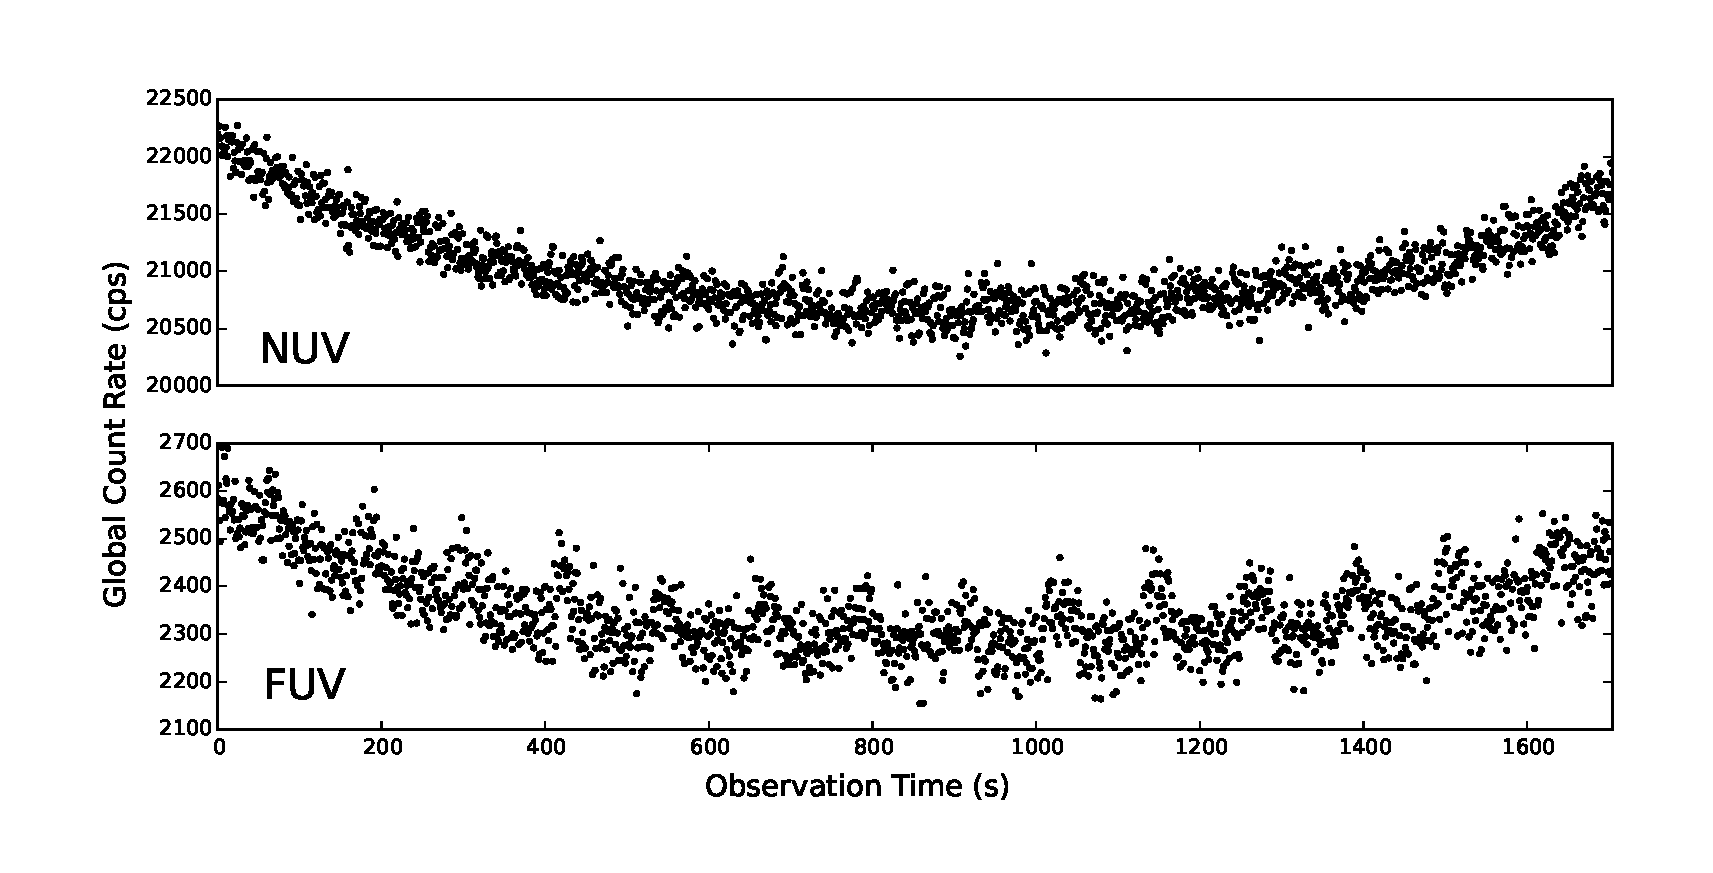
\includegraphics[scale=0.31]{gcr_smiley.eps}
\caption{Over the course of a typical eclipse such as this one, the global count rate falls and then rises in a characteristic ``smiley face'' pattern due to light scattered by Earth's atmosphere. The scalloped, periodic variations throughout the eclipse are due to the dither pattern moving the spacecraft minutely, repeatedly toward and away from the Earth's limb during an eclipse.\label{smiley}}
\end{figure}

\begin{figure}
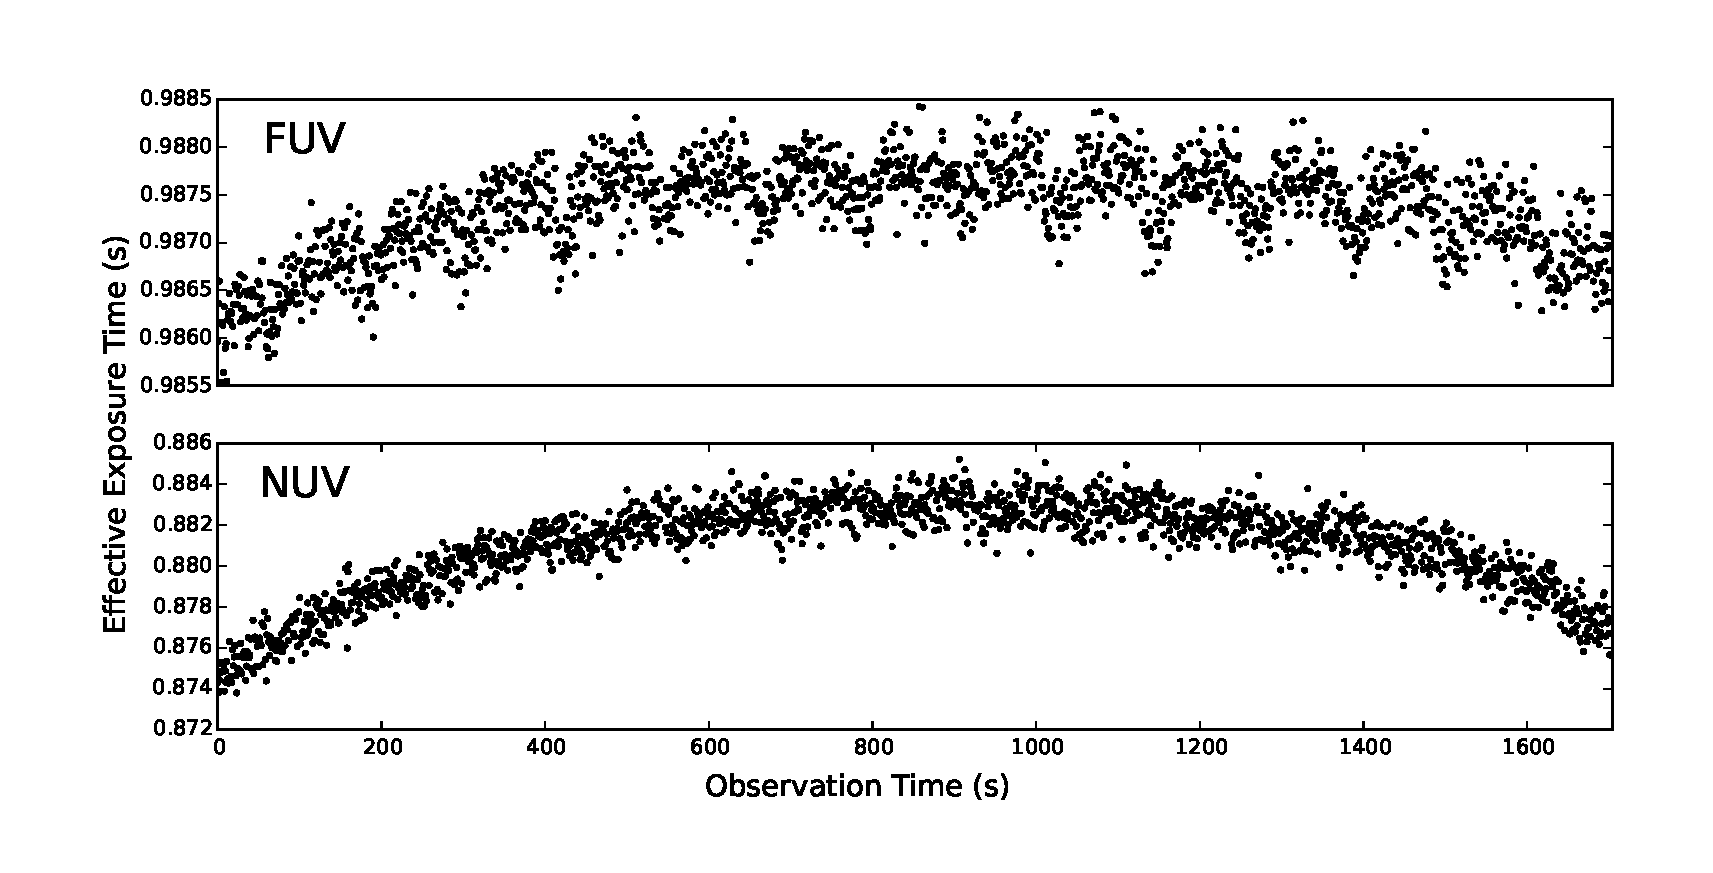
\includegraphics[scale=0.31]{expt_frowny.eps}
\caption{Detector dead time varies directly as a function of global count rate, so effective exposure time varies inversely. The scalloped, periodic variations throughout the eclipse are due to the dither pattern moving the spacecraft minutely, repeatedly toward and away from the Earth's limb during an eclipse.\label{frowny}}
\end{figure}

Note that the ratio of effective exposure time to raw exposure time is not constant over any finite period. Global count rate can change quite substantially, even during an observation of a single target, because the detector FOV is constantly moving in relationship to the sky, causing small changes in the global count rate due to field brightness changes. At the same time, the spacecraft is traveling through the shadow of the Earth and encountering shifts in ambient brightness due to airglow which likewise manifest as changes in global count rate. If one plots global count rates as a function of time for a typical 1600 second MIS observation, there will be a characteristic, broad parabolic shape (``smiley face''). (Fig.\ \ref{smiley}) This shape is inverted in a plot of effective exposure time as a function of the observing timestamps, because higher global count rates create more detector dead time, resulting in less effective exposure time. (Fig.\ \ref{frowny}) Researchers interested in the variability of targets within single observations should re-compute the exposure time for every bin in order to account for this effect. gAperture makes this correction automatically when creating a light curve.

\subsection{Background Correction}
There are currently two methods gAperture uses to correct for background flux.  The first method is a simple annulus estimation method where the total surface flux within an annulus surrounding the extraction aperture is scaled to the area of the aperture and subtracted. This method can be biased by the presence of relatively bright sources either within or near the annulus, although the bias can sometimes be mitigated by careful selection of annulus parameters (and assuming that the field is not crowded). The direct annulus method has the benefit of correcting for changing local background over an observation due to zodiacal light or airglow. It produces good agreement with Merged Catalog (MCAT) values for integrations of AIS depth or longer, on average, but with a larger dispersion likely due to brighter stars that are in or near the annulus contributing to an erroneously high background estimate.

The second method is to estimate the local sky background based upon backgrounds of nearby sources as reported in the official GALEX source catalog (MCAT). In this method, the coadd MCAT is searched for sources within a small region of the target position. The arithmetical mean of reported flux of all returned MCAT entries is then used as the estimated background at the target location. As one might expect, this method results in gAperture fluxes that are in good agreement with the MCAT on average, and with good dispersion, but does not correct for either inter- or intra-visit variations in the sky background.

We suggest that the first method be used for studies of intra-visit variability. The second method may be useful for researchers wishing to compare gPhoton results to previous work that used data from the GALEX catalogs. Note that the first method could also produce false variability if the source(s) in the aperture are not changing, but one or more sources in or near the annulus are.  When this is a possibility, we suggest that researchers check the MCAT as well as a gMap-produced image of the targeted region for nearby sources, and run an independent photometric analysis for those.

We also tested two variations of the annulus method that might mitigate the presence of stars in or near the background annulus, both of which were abandoned because they produced poor agreement with catalog fluxes and they were highly sensitive to somewhat arbitrary input parameters. The first method, which we called ``swiss cheese'', mimicked that applied by Morrissey in the analysis of the GALEX standard star LDS749B \citet{mor2007}: nearby bright stars from the MCAT out to several sigma, assuming Gaussian profiles, were masked out by excluding those data and sky regions from subsequent calculations. The second method was a direct port of the ``sigma clipping'' algorithm used by the mission pipeline as described in \url{http://www.galex.caltech.edu/DATA/gr1_docs/Background_determination_and_source_extraction_for_GALEX_data.pdf}, which iteratively excluded and interpolated over relatively bright regions (i.e. "sigma clipping"), using full Poissonian statistics to account for low, diffuse UV background.

\subsection{Relative Response Correction}
In the mission pipeline, differential sensitivity ("response") across the detector was corrected for by the application of relative response maps. These relative response maps (-rrhr) were composed of successive projections of an upsampled detector flat on the sky in second increments, weighted for effective exposure time over those increments, which could then be divided out of the integrated count maps over the same time range to produce fully calibrated intensity maps (-int). In developing gPhoton, we discovered that not only did this repeated interpolation unnecessarily degrade the information in the flat, but it was also computationally intensive and slow. For this reason, we apply the flat at the detector level by weighting each individual photon event by the value of the pixel in the flat field that corresponds to the detector location at which the event was recorded. The exposure time correction is performed as a separate step.

\subsection{Flux Uncertainties}
The flux uncertainties produced by gAperture are computed by adding the counting error in the aperture and background annulus in quadrature. If there are relatively bright sources in the background annulus, then this will be an underestimate.

\section{Calibration Tests}
\label{calibration}

We performed both relative and absolute tests of gAperture performance, comparing output respectively to that of the mission pipeline (as recorded in the MCAT) and to the white dwarf calibration standard stars LDS749B and LB227. In all cases of relative comparisons against the MCAT, source position on the sky and time ranges for detected sources were passed directly to gAperture on a per-visit basis. To allow direct comparison, a photometric aperture of 6 arcseconds was used, equivalent to the MCAT \emph{APER4} column. The gAperture background annulus was defined to extend from 30 to 90 arcseconds. When appropriate, source brightnesses were aperture corrected using the table defined in Figure 4 of \cite{mor2007}. Except where noted, source positions were determined by using a random number generator to select right ascension and declination positions on the sky as the center position of a 0.1 degree cone search of the MCAT sources. All available visits for any sources within the cone and brighter than the threshold AB magnitude of 20 were then used for analysis, excluding sources for which there was a total raw exposure time of greater than 5000 seconds to avoid biasing the analysis with a few very deep fields.

The aperture radius for absolute photometry using the white dwarf standards was set to 90 arcseconds, to capture the maximum amount of source flux, with a background annulus extending from 90 to 180 arcseconds and no aperture correction.

\subsection{Astrometric Reproducibility}
{\color{red}Graphic In Progress}
We compare the mean photon event position within the aperture to the MCAT source position for {\color{red}XXXX} randomly selected MCAT targets. One source of uncertainty here is that the center of brightness was calculated by the mission pipeline on a pixel-based map, whereas gPhoton uses the photons directly. Another possible source of error is that one should ideally fit a two-dimensional Gaussian bounded by an off-center circle to find the center of brightness.  {\color{red}Were the same sources selected from each band?  Did the sources sample different observing modes, times, sky coordinates?}  We find that nearly all sources lie within one GALEX resolution element ($\sim 6''$), and that \{{\color{red}XXXX, YYYY}\} lie within {\color{red}$XXXX''$} in the FUV and NUV bands, respectively (Fig.\ \ref{fuvnuvastrometry}).

\begin{figure}
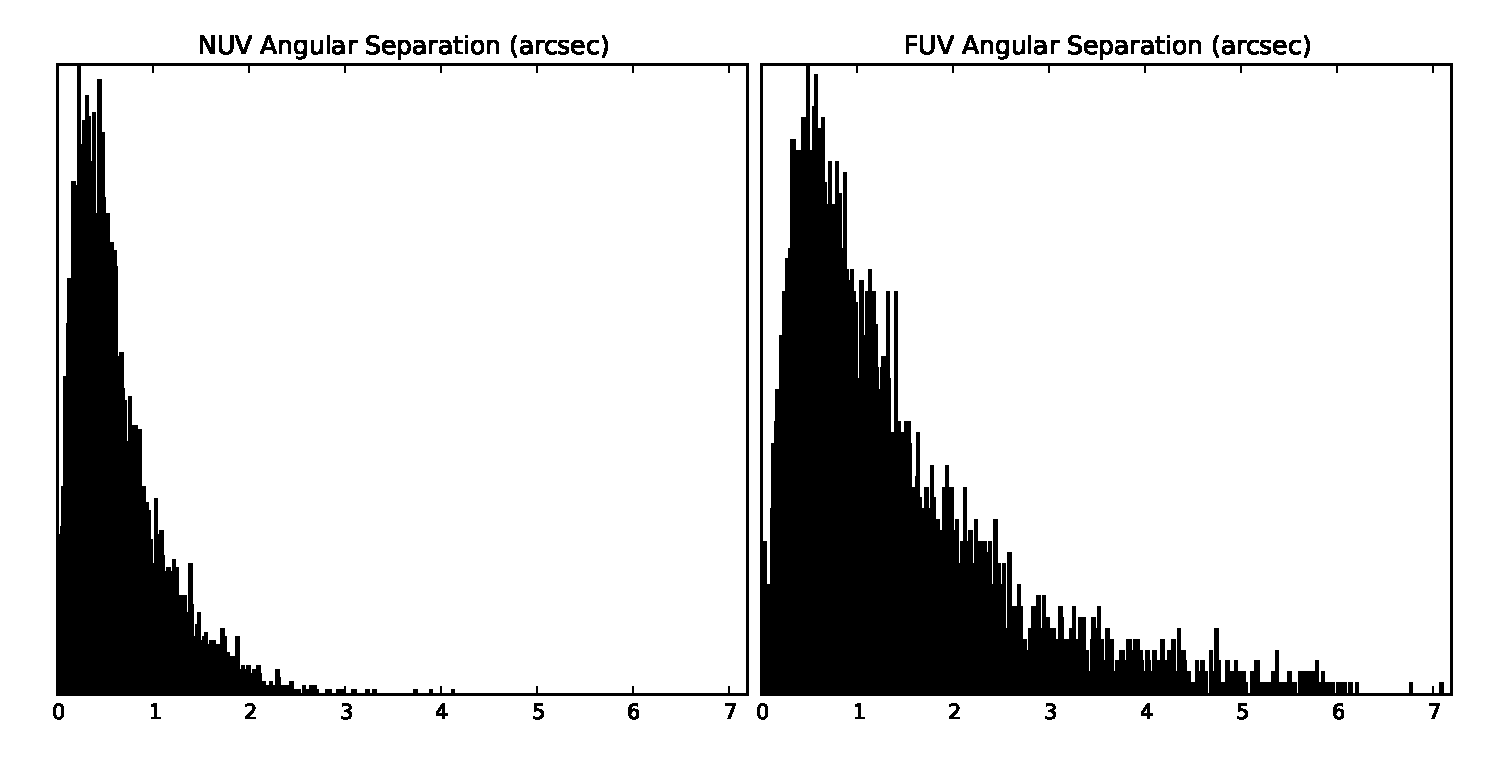
\includegraphics[scale=0.35]{FigAngSepFUVNUV.eps}
\caption{Angular separation between gPhoton and MCAT source positions for {\color{red}XXXX} MCAT sources in both bands. \label{fuvnuvastrometry}}
\end{figure}

\subsection{Relative Flux Precision}
As a test of the relative photometric precision from gPhoton, we plot the difference between the MCAT magnitude and gAperture magnitude against the MCAT magnitude for 7692 and 20213 randomly selected MCAT sources in FUV and NUV respectively. Fig.\ \ref{fuvrelphot} and Fig.\ \ref{nuvrelphot} use the background estimated from the gAperture background annulus, while Fig.\ \ref{fuvrelphotmcat} and Fig.\ \ref{nuvrelphotmcat} use the per-visit MCAT background. To a first-order approximation, Although both methods show good agreement on average, with higher dispersion for lower source brightnesses, the MCAT background method has a more symmetric distribution overall. The asymmetry of the annulus background method as compared to the per-visit MCAT is highlighted in Fig.\ \ref{bgrelphot} and likely due to unmasked background sources in the annulus, which effect is more severe in NUV than FUV due to higher source densities.



\begin{figure}
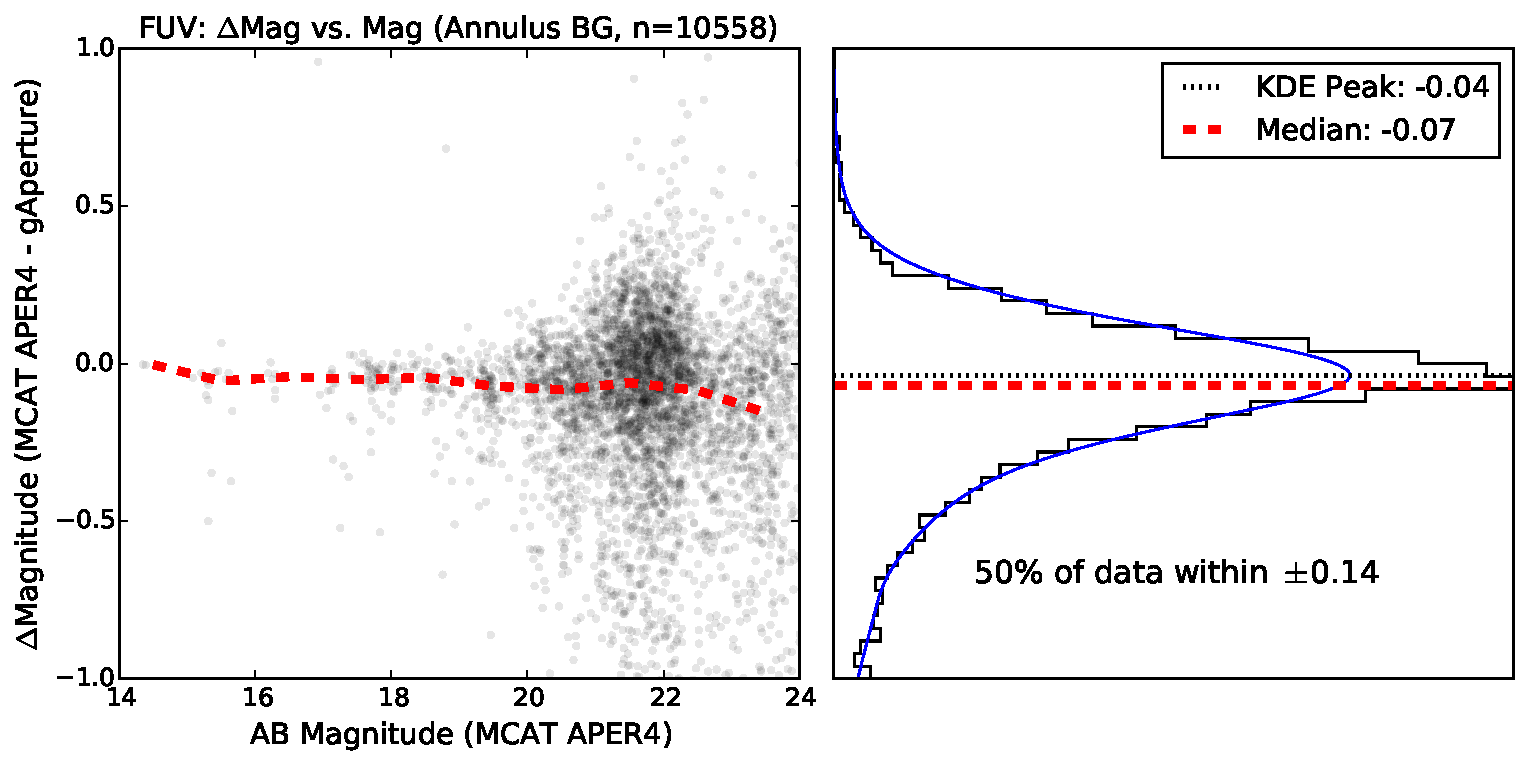
\includegraphics[scale=0.32]{FigRelPhotFUV-annulus_bg.pdf}
\caption{Comparison between MCAT and gPhoton FUV fluxes, using backgrounds estimated from unmasked annuli, for 7692 randomly selected MCAT sources. The dashed line denotes the median difference in half magnitude bins. 
\label{fuvrelphot}}
\end{figure}

\begin{figure}
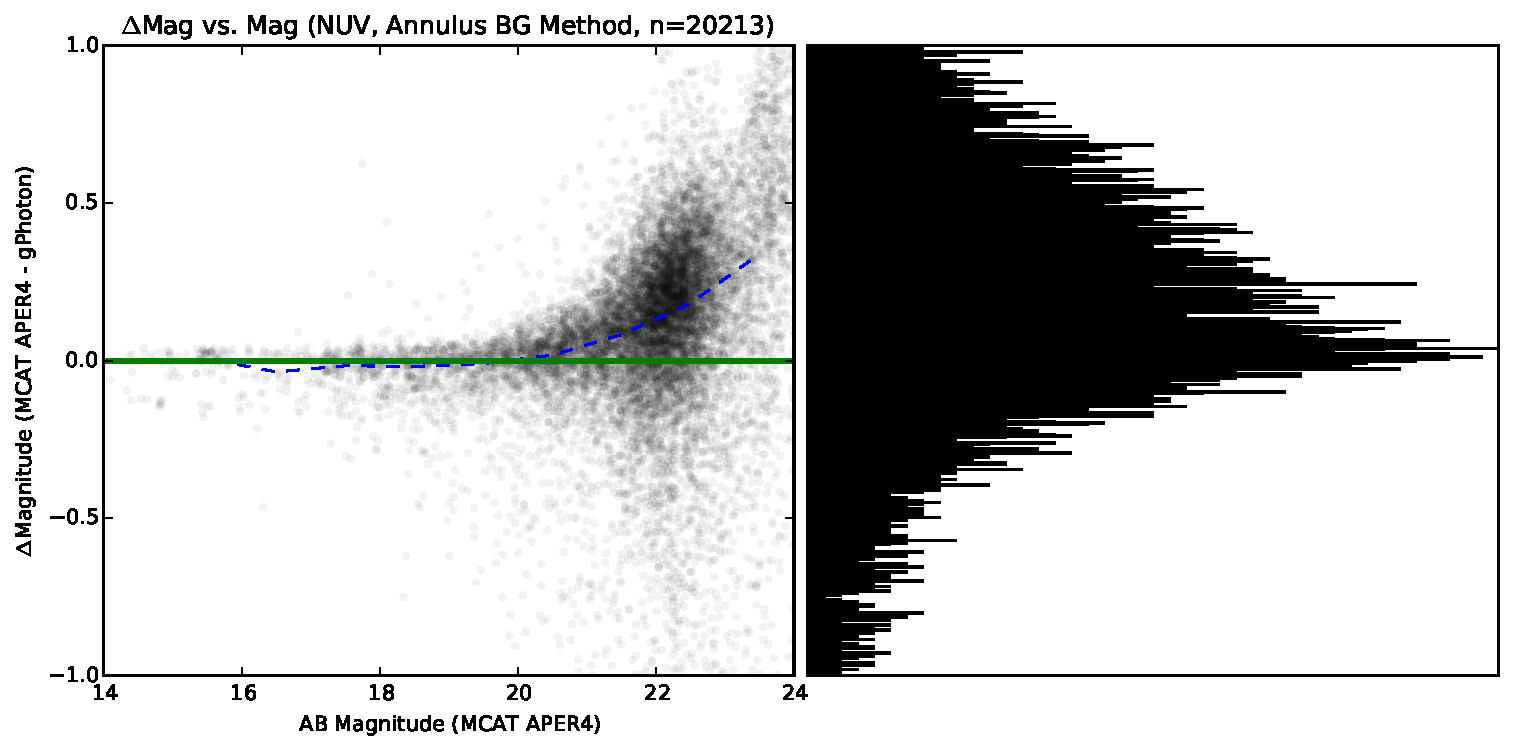
\includegraphics[scale=0.32]{FigRelPhotNUV-annulus_bg.pdf}
\caption{Comparison between MCAT and gPhoton NUV fluxes, using backgrounds estimated from unmasked annuli, for 20213 randomly selected MCAT sources. The dashed line denotes the median difference in half magnitude bins.
\label{nuvrelphot}}
\end{figure}

\begin{figure}
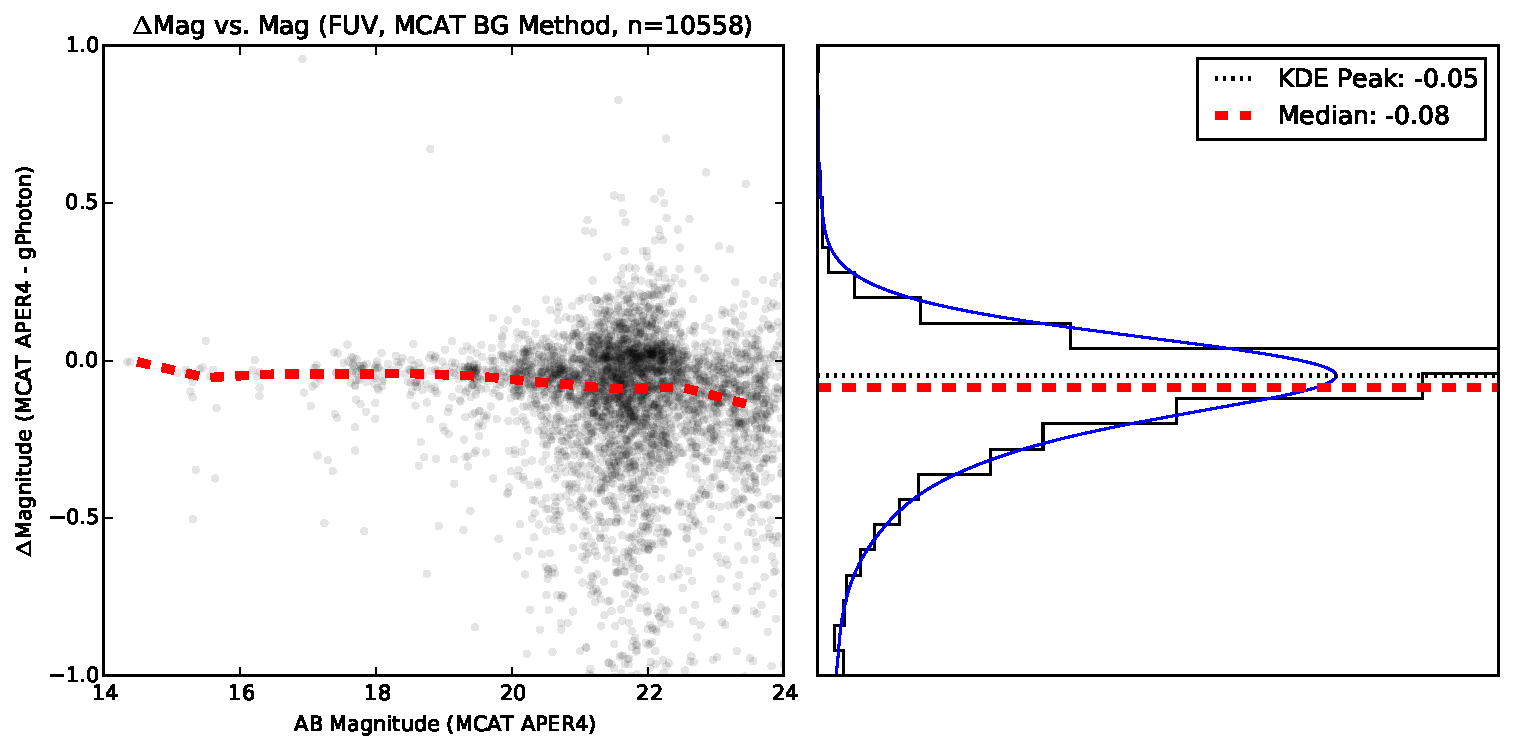
\includegraphics[scale=0.32]{FigRelPhotFUV-mcat_bg.pdf}
\caption{omparison between MCAT and gPhoton FUV fluxes, using background estimates drawn from the visit-level MCAT, for 7692 randomly selected MCAT sources. The dashed line denotes the median difference in half magnitude bins.
\label{fuvrelphotmcat}}
\end{figure}

\begin{figure}
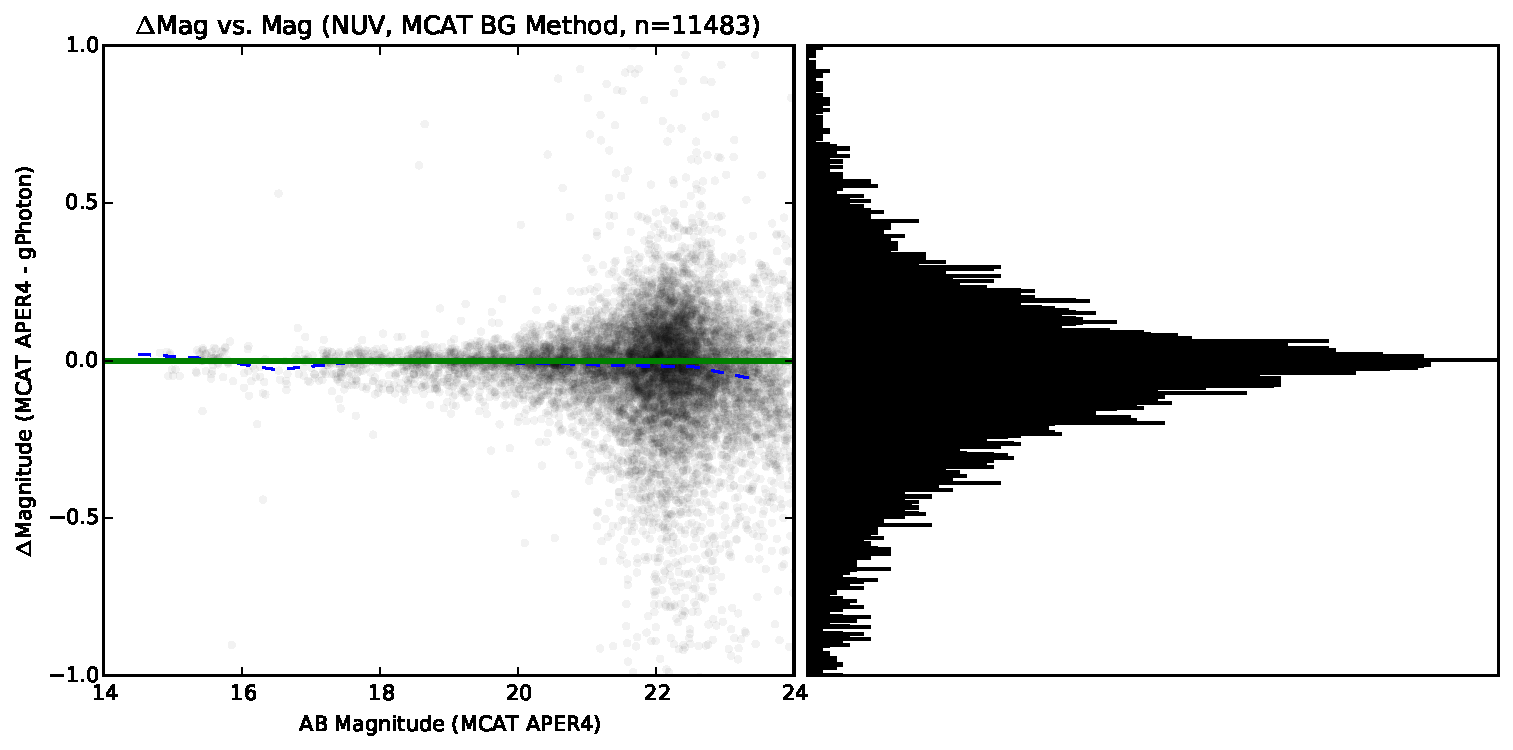
\includegraphics[scale=0.32]{FigRelPhotNUV-mcat_bg.pdf}
\caption{Comparison between MCAT and gPhoton NUV fluxes, using background estimates drawn from the visit-level MCAT, for 20213 randomly selected MCAT sources. The dashed line denotes the median difference in half magnitude bins.
\label{nuvrelphotmcat}}
\end{figure}

\begin{figure}
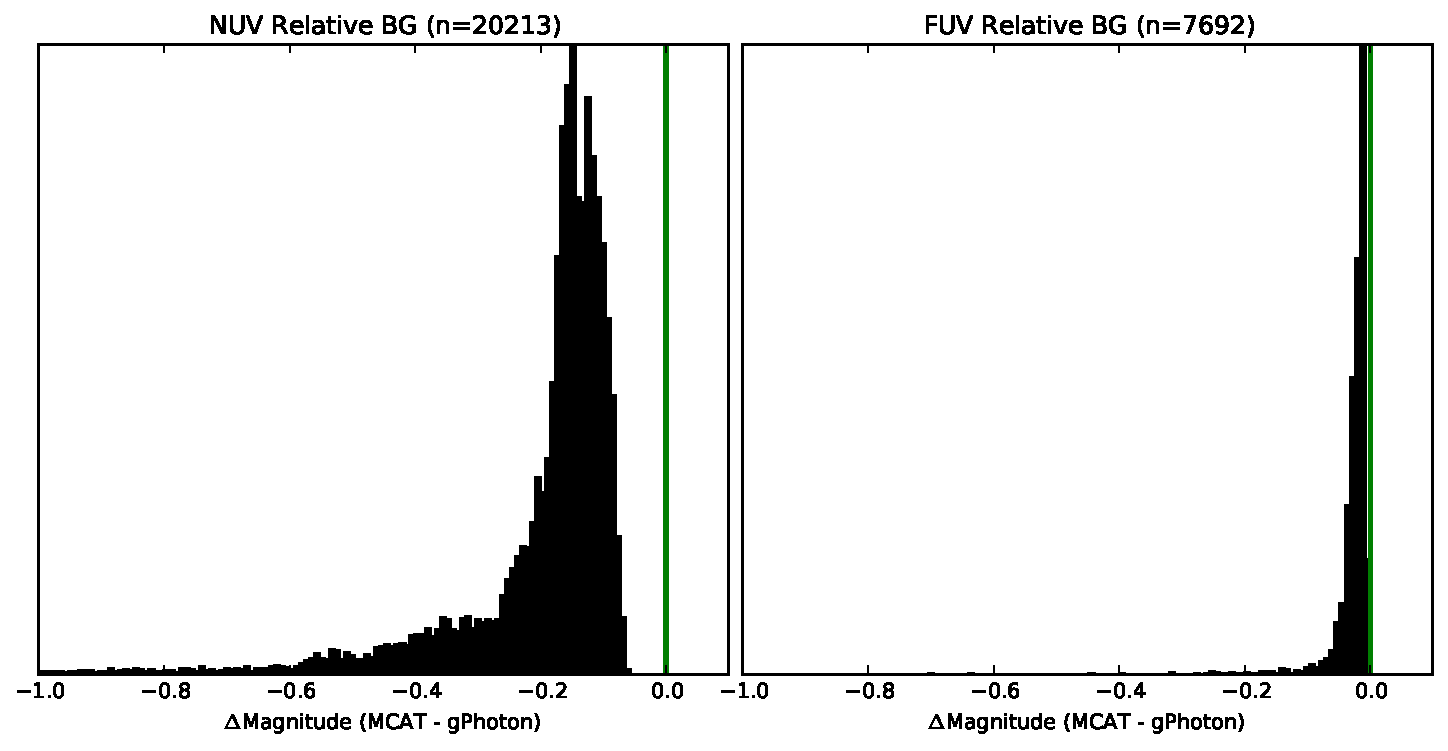
\includegraphics[scale=0.32]{BG_dMag.pdf}
\caption{Effective surface brightness within a 6 arcsecond aperture for the gAperture unmasked annulus method of background estimation as compared to estimates drawn from visit-level MCAT.
\label{bgrelphot}}
\end{figure}

\begin{figure}
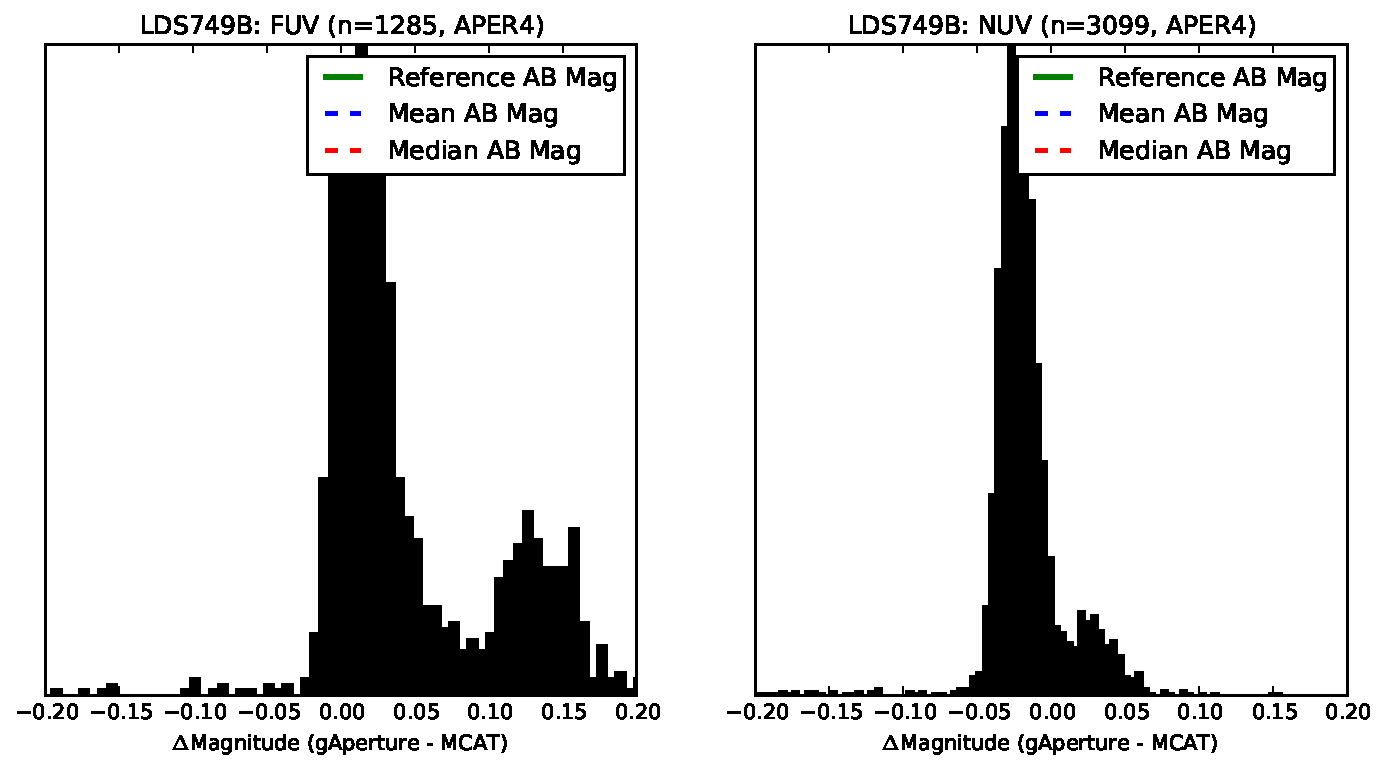
\includegraphics[scale=0.32]{dMag_LDS749B.pdf}
\caption{The relative photometry of LDS749B from gAperture compared against the mission produced catalog values, using an aperture equivalent to the MCAT APER4 column. The distribution in both bands is clearly bimodal. The small mode in NUV is strongly correlated to data collected after the CSP event. We have not been able to understand the source of the bimodality in FUV but, importantly, it does not show up in other relative photometry, including of LB227, so it is likely due to something unique about LDS749B observations.
\label{ldsrelphot}}
\end{figure}

\begin{figure}
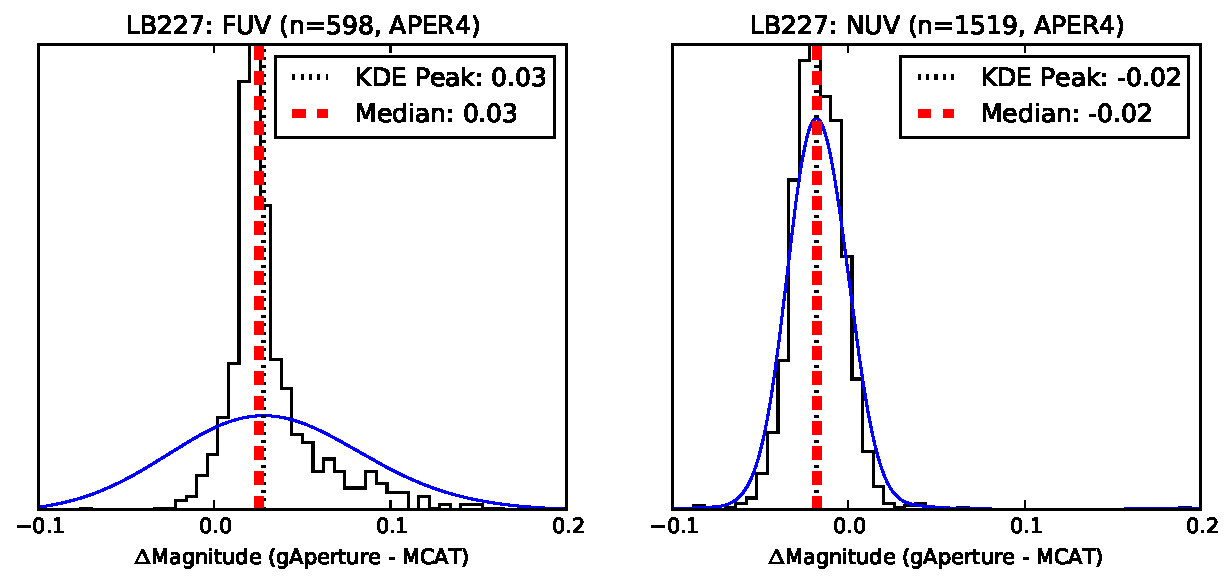
\includegraphics[scale=0.32]{dMag_LB227.pdf}
\caption{The relative photometry of LB227 from gAperture compared against the mission produced catalog values, using an aperture equivalent to the MCAT APER4 column.
\label{lbrelphot}}
\end{figure}


\subsection{Absolute Flux Precision}
As described in \citet{mor2007}, the primary calibration standard star of choice for GALEX was the white dwarf LDS749B, which is also one of the Hubble Space Telescope standards. A total of \{259909, 595672\} seconds of exposure depth in the FUV and NUV bands, respectively, were made on this source. We use gAperture to compute magnitudes for all of these observations in both bands and compare them against the standard magnitudes used by GALEX (Fig.\ \ref{ldsabsphot}). We measure fluxes separated into visit levels to match the exposure times in the MCAT.

All visit-level MCAT detections within 0.001 degrees of the nominal source position for each source were used as the basis to generate gAperture photometry over matching time ranges and at matching sky positions. We used a photometric aperture with a 0.025 degree (90 arcsecond) radius and an annulus extending from 0.025 to 0.05 degrees. The particularly large aperture corresponds to the largest custom aperture used by \cite{mor2007} to enclose the maximum amount of flux, and the substantial annulus is only contaminated by a small number of relatively faint (>20 AB Mag) stars.

\begin{figure}
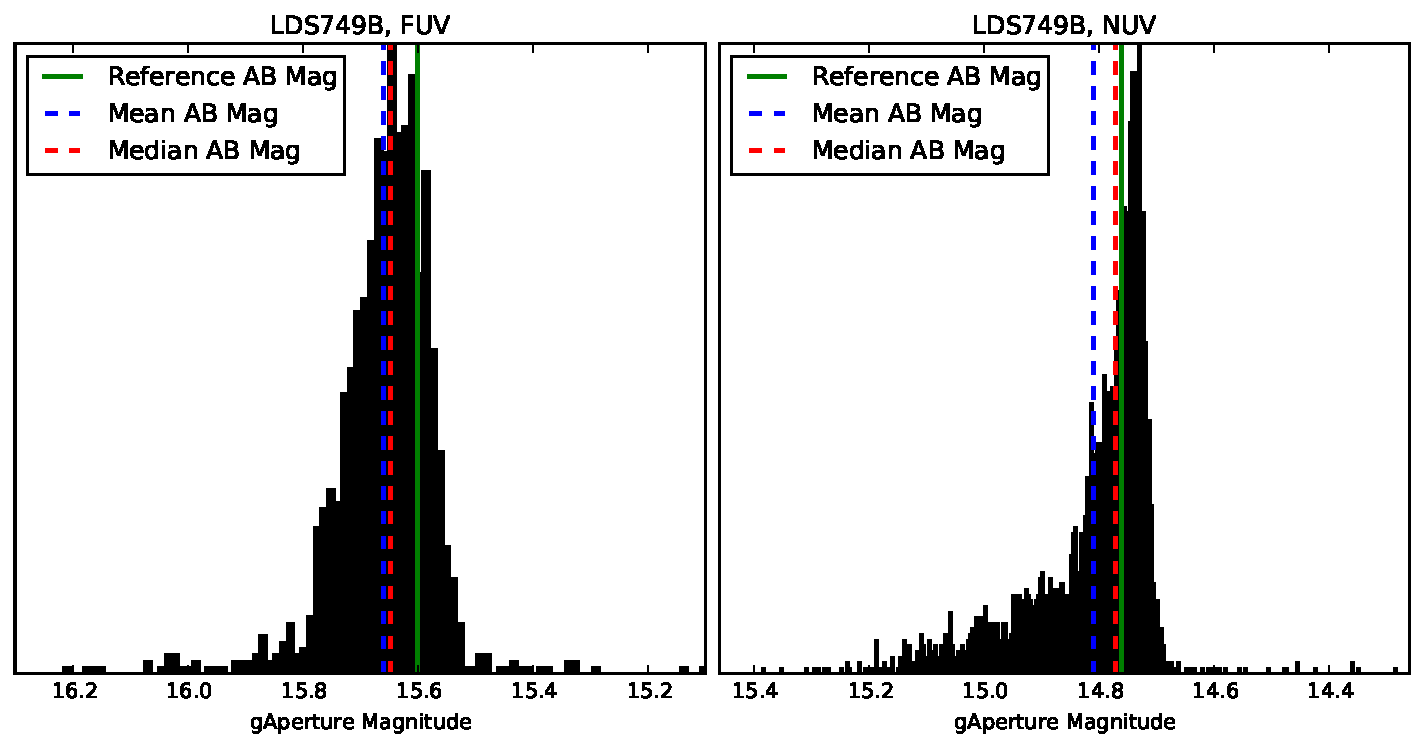
\includegraphics[scale=0.35]{LDS749B_ABMag_dist.pdf}
\caption{These histograms show the differences, in AB magnitude, between background subtracted photometry of LDS749B produced by gAperture and the mission pipeline. Aperture radii of six seconds of arc (equivalent to the MCAT \emph{APER4} column) were used, with the background estimated within an annulus extending between 30 to 90 arcseconds from the source position.
\label{ldsrelphot}}
\end{figure}

\begin{figure}
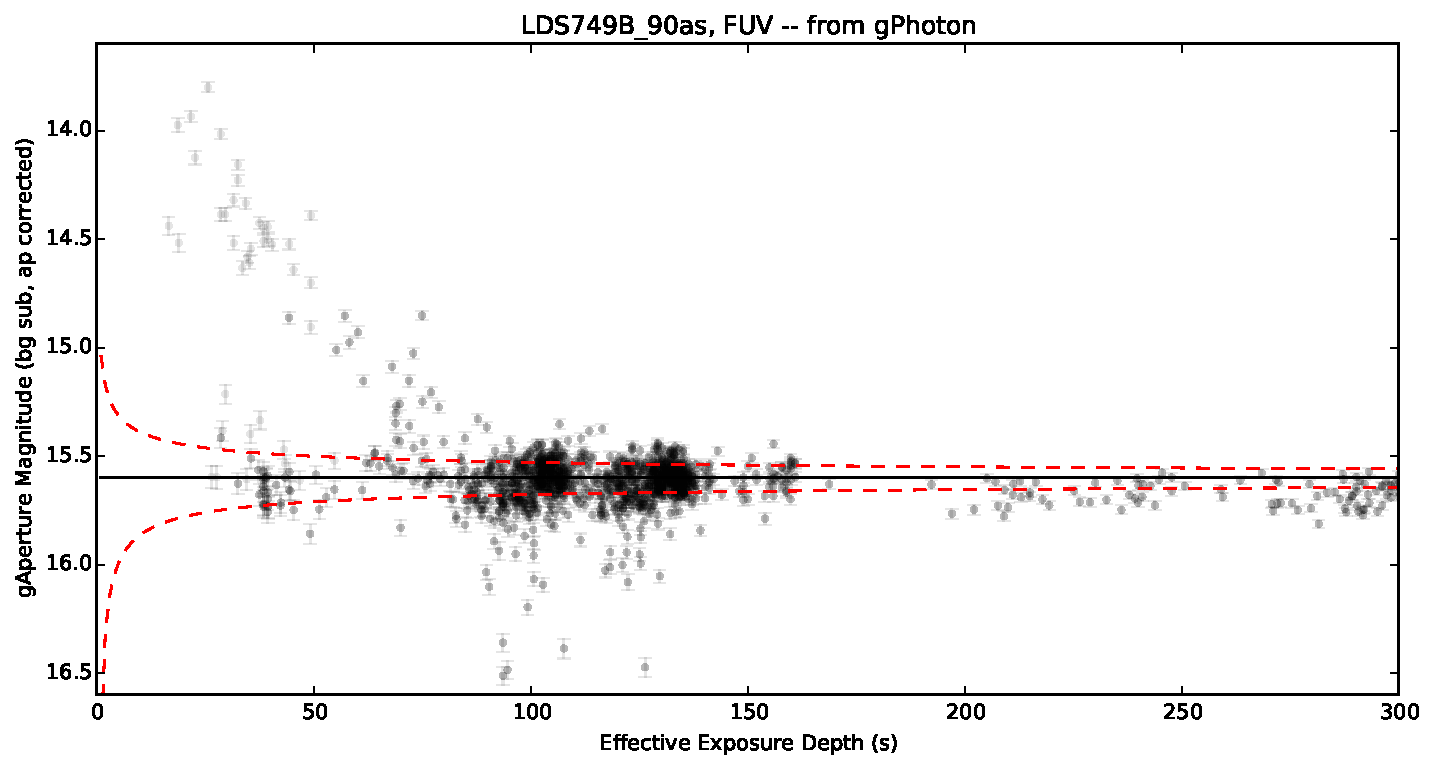
\includegraphics[scale=0.35]{LDS749B_90as_ABMag_FUV.pdf}
\caption{Comparison of gPhoton FUV fluxes for LDS749B to the catalog reference value of 15.57 AB Mag (solid line) as a function of exposure depth. The aperture had a radius of 90 arcseconds and backgrounds were estimated with an unmasked annulus extending from 90 to 180 arcseconds. The dashed lines denote ideal 3 sigma scatter as predicted from counting statistics. The error bars on the points denote 1 sigma.
\label{ldsabsphotfuv}}
\end{figure}

\begin{figure}
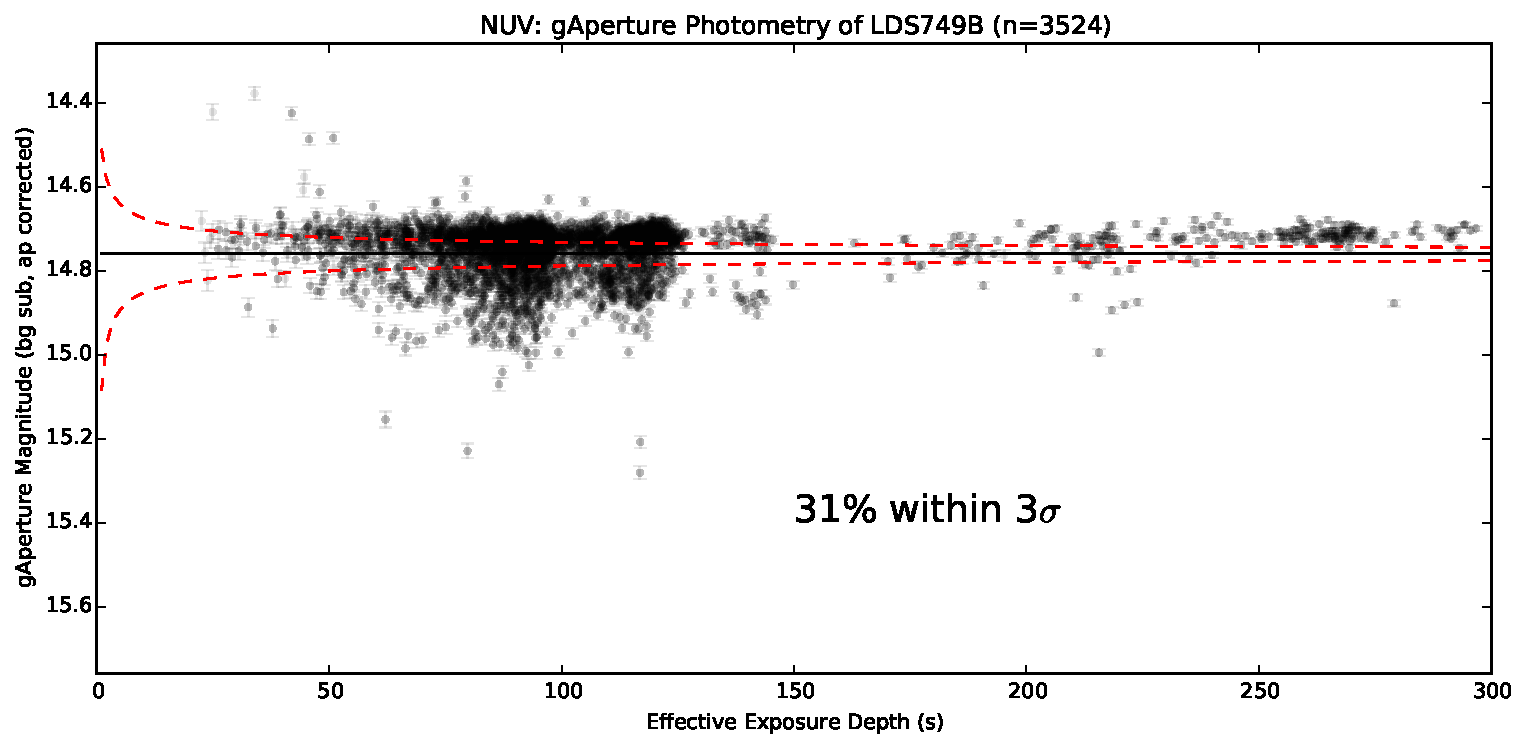
\includegraphics[scale=0.35]{LDS749B_90as_ABMag_NUV.pdf}
\caption{Comparison of gPhoton NUV fluxes for LDS749B to the catalog reference value of 14.71 AB Mag (solid line) as a function of exposure depth. The aperture had a radius of 90 arcseconds and backgrounds were estimated with an unmasked annulus extending from 90 to 180 arcseconds. The dashed lines denote ideal 3 sigma scatter as predicted from counting statistics. The error bars on the points denote 1 sigma.
\label{ldsabsphotnuv}}
\end{figure}

\begin{figure}
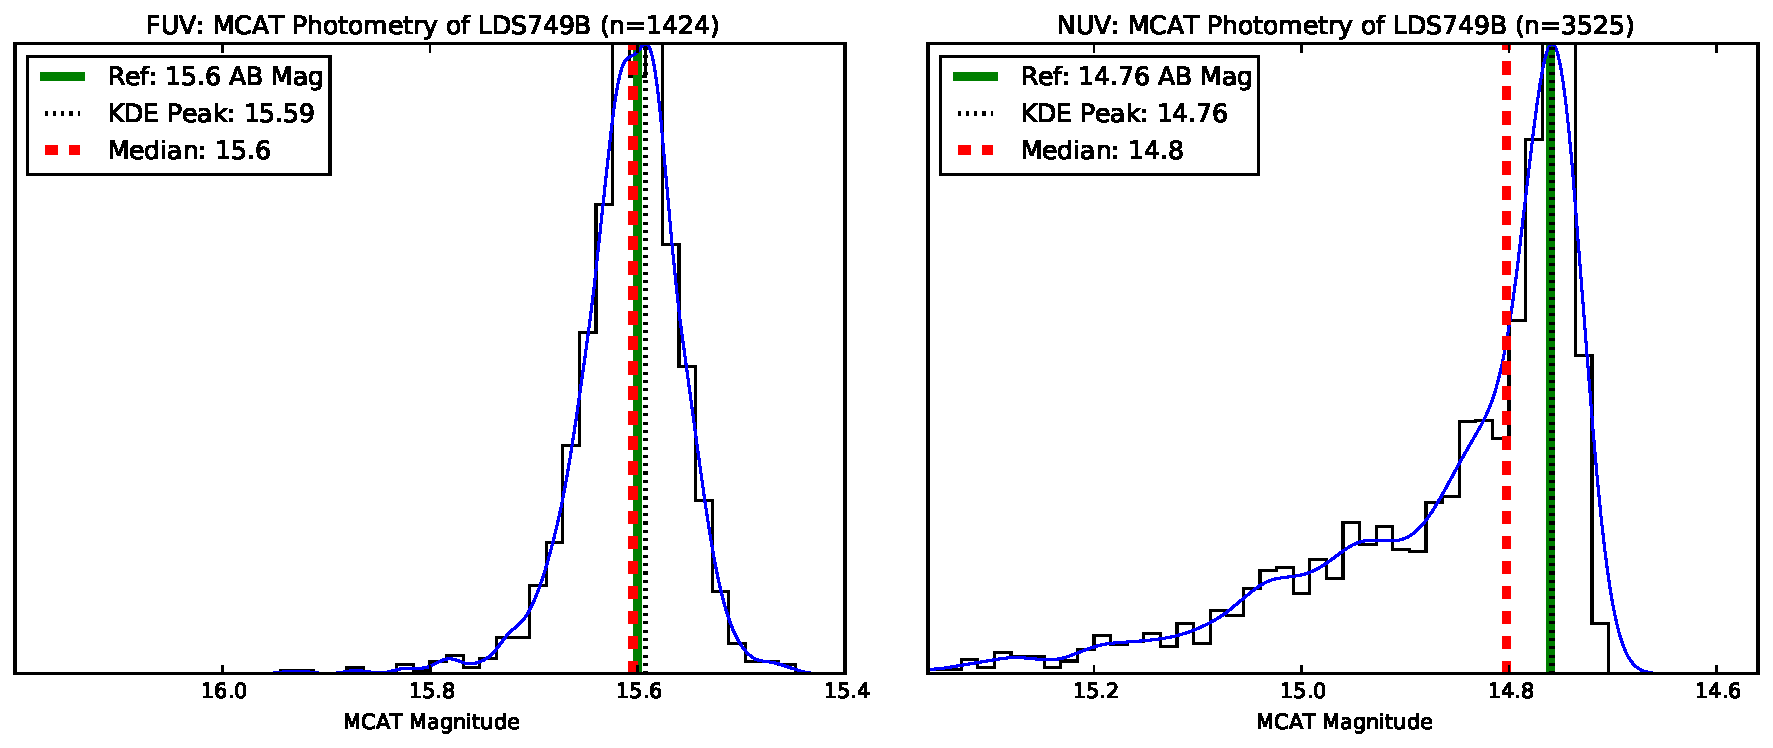
\includegraphics[scale=0.35]{LDS749B_ABMag_dist_MCAT.pdf}
\caption{These histograms show the differences, in AB magnitude, between background subtracted photometry of LDS749B produced by gAperture and the mission pipeline. Aperture radii of six seconds of arc (equivalent to the MCAT \emph{APER4} column) were used, with the background estimates drawn from the visit-level MCAT.
\label{ldsrelphotmcat}}
\end{figure}

\begin{figure}
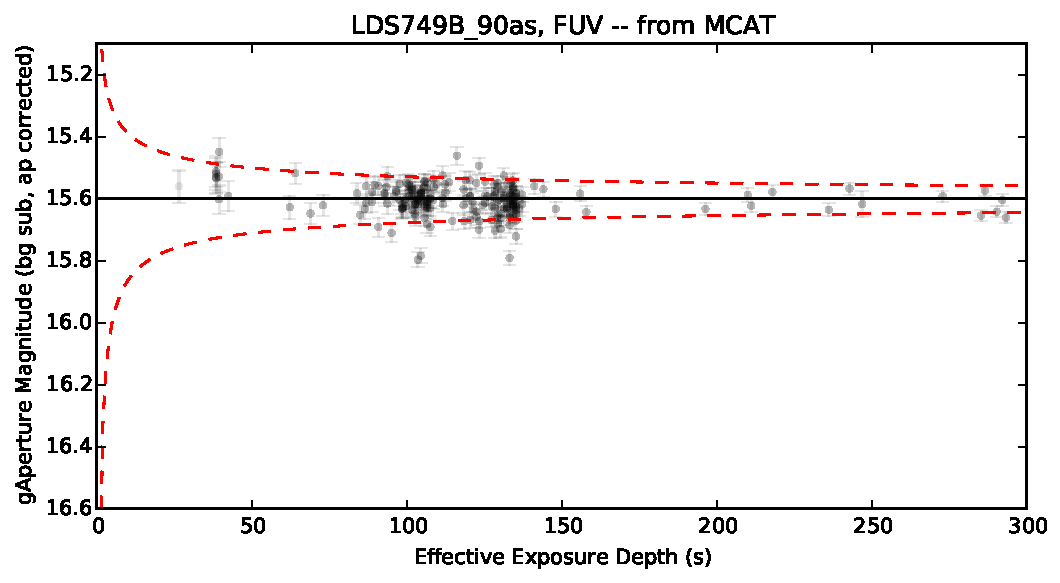
\includegraphics[scale=0.35]{LDS749B_90as_ABMag_FUV_MCAT.pdf}
\caption{Comparison of gPhoton FUV fluxes for LDS749B to the catalog reference value of 15.57 AB Mag (solid line) as a function of exposure depth. The aperture had a radius of 90 arcseconds and backgrounds estimates were drawn from the visit-level MCAT. The dashed lines denote ideal 3 sigma scatter as predicted from counting statistics. The error bars on the points denote 1 sigma.
\label{ldsabsphotfuvmcat}}
\end{figure}

\begin{figure}
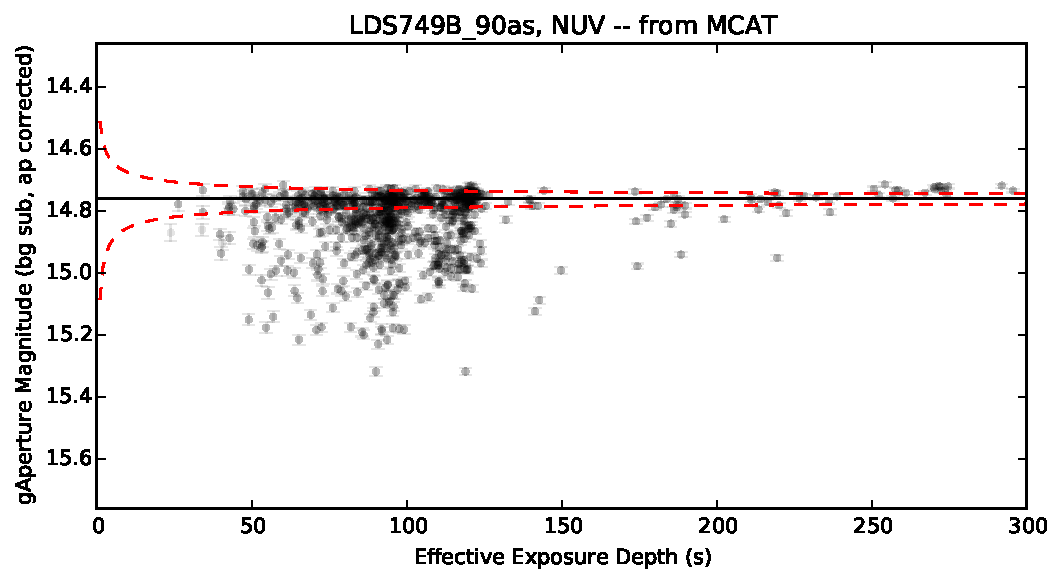
\includegraphics[scale=0.35]{LDS749B_90as_ABMag_NUV_MCAT.pdf}
\caption{Comparison of gPhoton NUV fluxes for LDS749B to the catalog reference value of 14.71 AB Mag (solid line) as a function of exposure depth. The aperture had a radius of 90 arcseconds and background estimates drawn from the visit-level MCAT. The dashed lines denote ideal 3 sigma scatter as predicted from counting statistics. The error bars on the points denote 1 sigma.
\label{ldsabsphotnuvmcat}}
\end{figure}

\begin{figure}
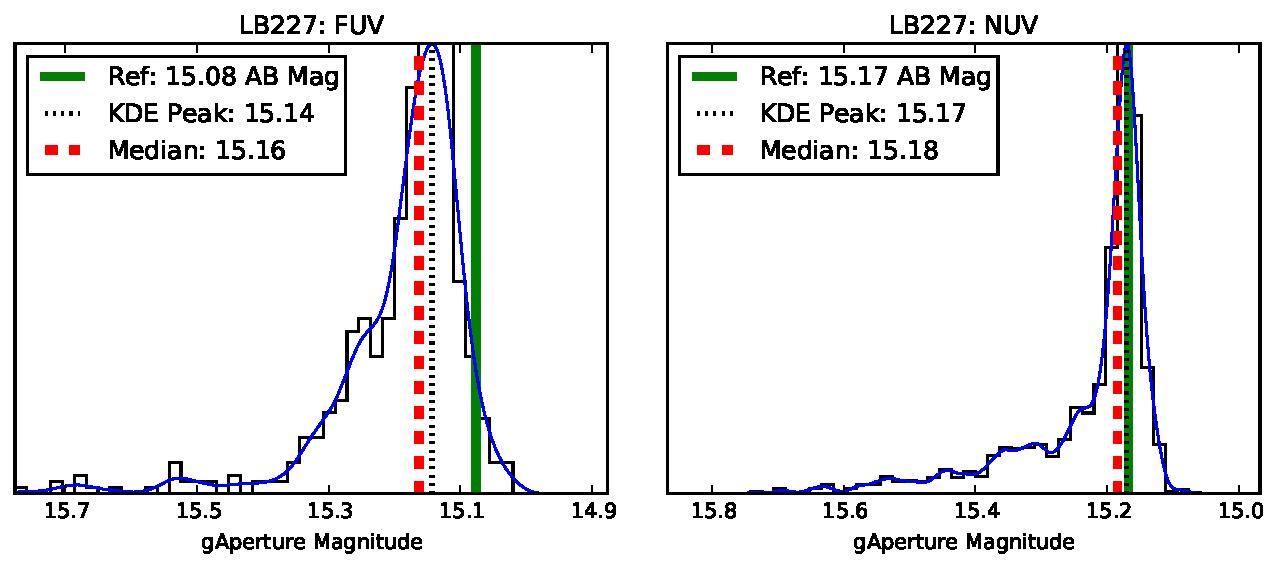
\includegraphics[scale=0.35]{LB227_ABMag_dist.pdf}
\caption{These histograms show the differences, in AB magnitude, between background subtracted photometry of LB227 produced by gAperture and the mission pipeline. Aperture radii of six seconds of arc (equivalent to the MCAT \emph{APER4} column) were used, with the background estimated within an annulus extending between 30 to 90 arcseconds from the source position. {\color{red}Still working on this graphic.}
\label{ldsrelphot}}
\end{figure}

\begin{figure}
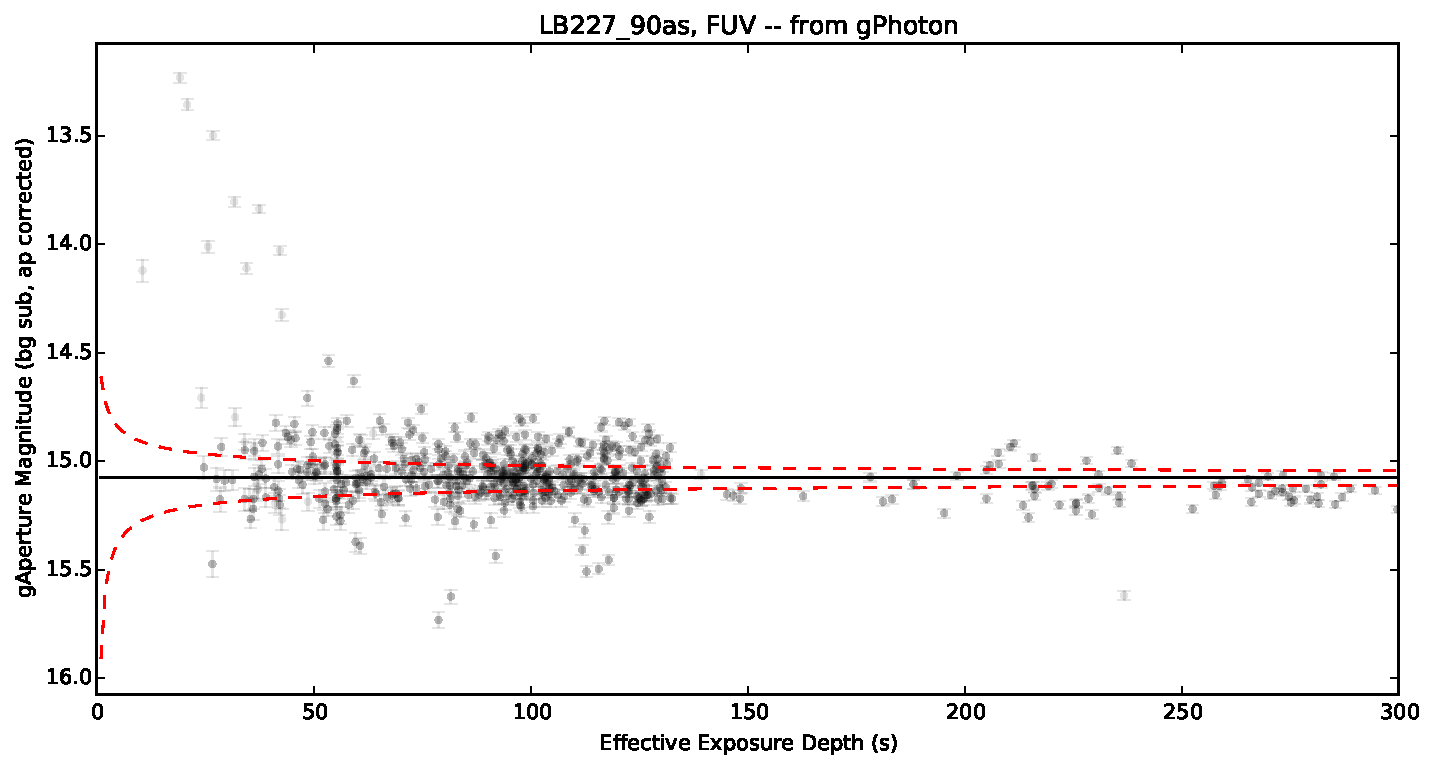
\includegraphics[scale=0.35]{LB227_90as_ABMag_FUV.pdf}
\caption{Comparison of gPhoton FUV fluxes for LB227 to the catalog reference value of 15.076 AB Mag (solid line) as a function of exposure depth. The aperture had a radius of 90 arcseconds and backgrounds were estimated with an unmasked annulus extending from 90 to 180 arcseconds. The dashed lines denote ideal 3 sigma scatter as predicted from counting statistics. The error bars on the points denote 1 sigma.
\label{ldsabsphotfuv}}
\end{figure}

\begin{figure}
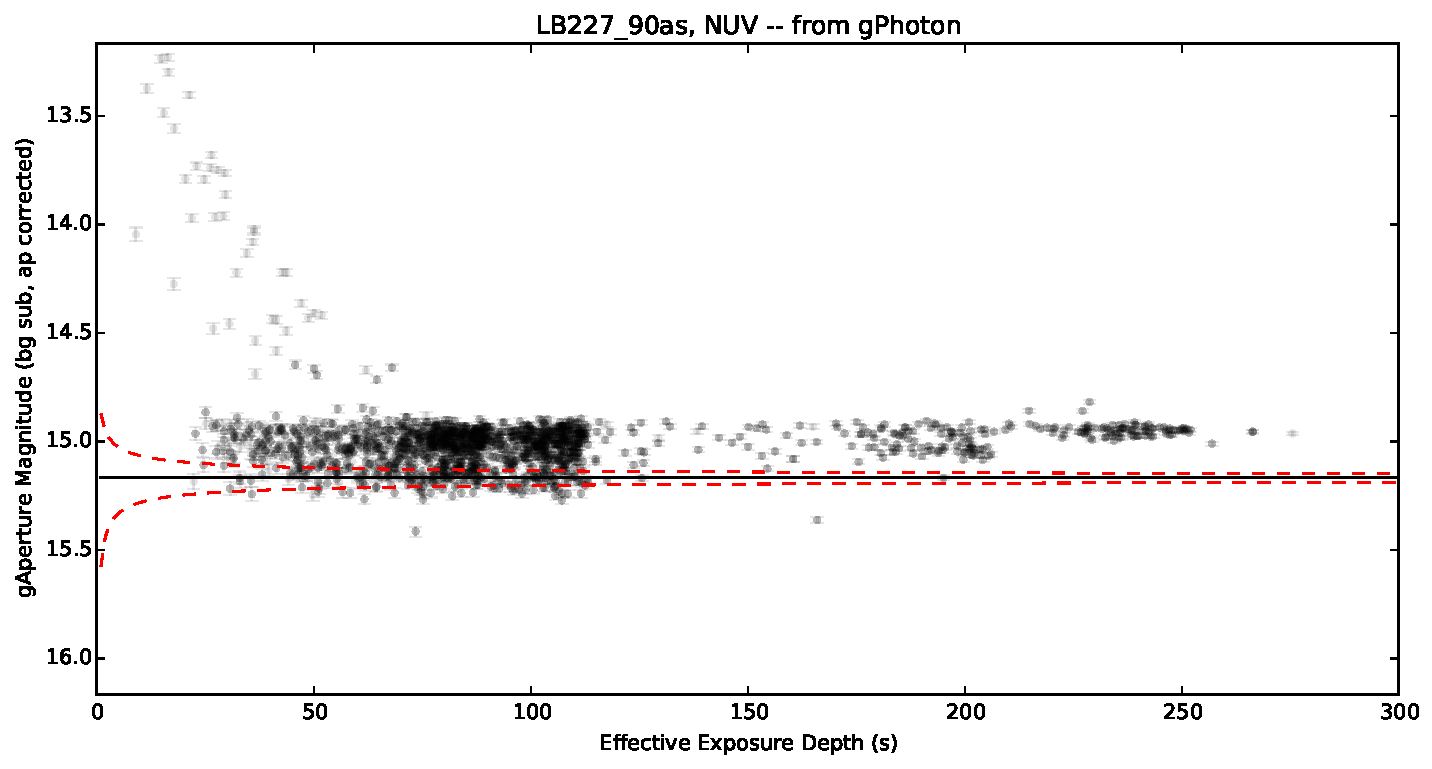
\includegraphics[scale=0.35]{LB227_90as_ABMag_NUV.pdf}
\caption{Comparison of gPhoton NUV fluxes for LB227 to the catalog reference value of 15.168 AB Mag (solid line) as a function of exposure depth. The aperture had a radius of 90 arcseconds and backgrounds were estimated with an unmasked annulus extending from 90 to 180 arcseconds. The dashed lines denote ideal 3 sigma scatter as predicted from counting statistics. The error bars on the points denote 1 sigma.
\label{ldsabsphotnuv}}
\end{figure}

\begin{figure}
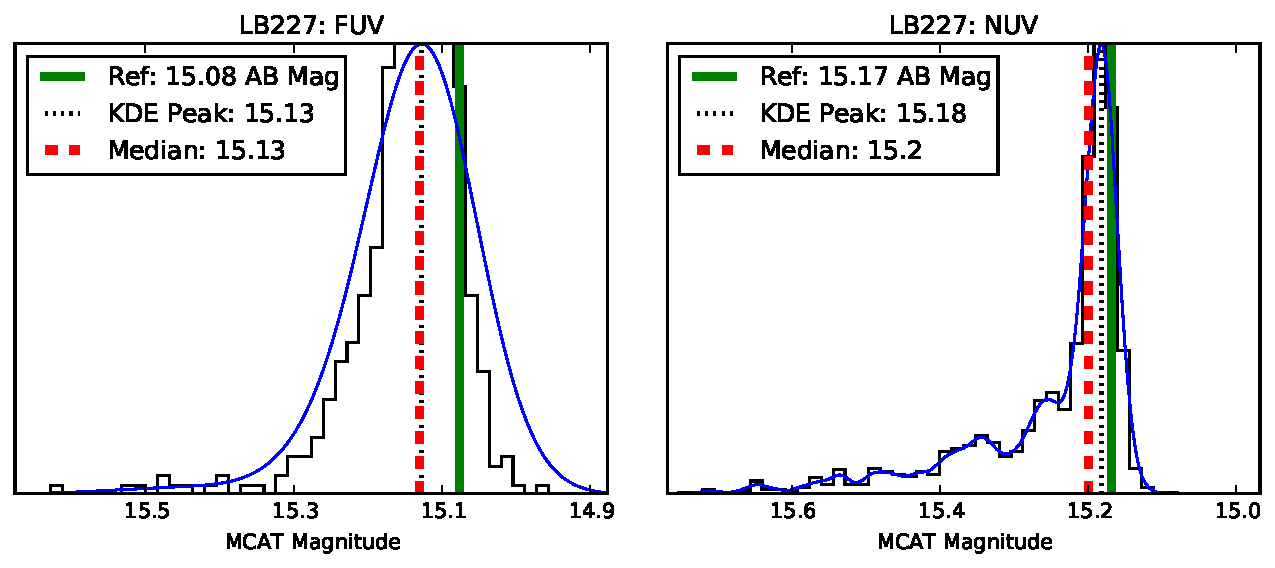
\includegraphics[scale=0.35]{LB227_ABMag_dist_MCAT.pdf}
\caption{These histograms show the differences, in AB magnitude, between background subtracted photometry of LB227 produced by gAperture and the mission pipeline. Aperture radii of six seconds of arc (equivalent to the MCAT \emph{APER4} column) were used, with the background estimates drawn from the visit-level MCAT.
\label{ldsrelphotmcat}}
\end{figure}

\begin{figure}
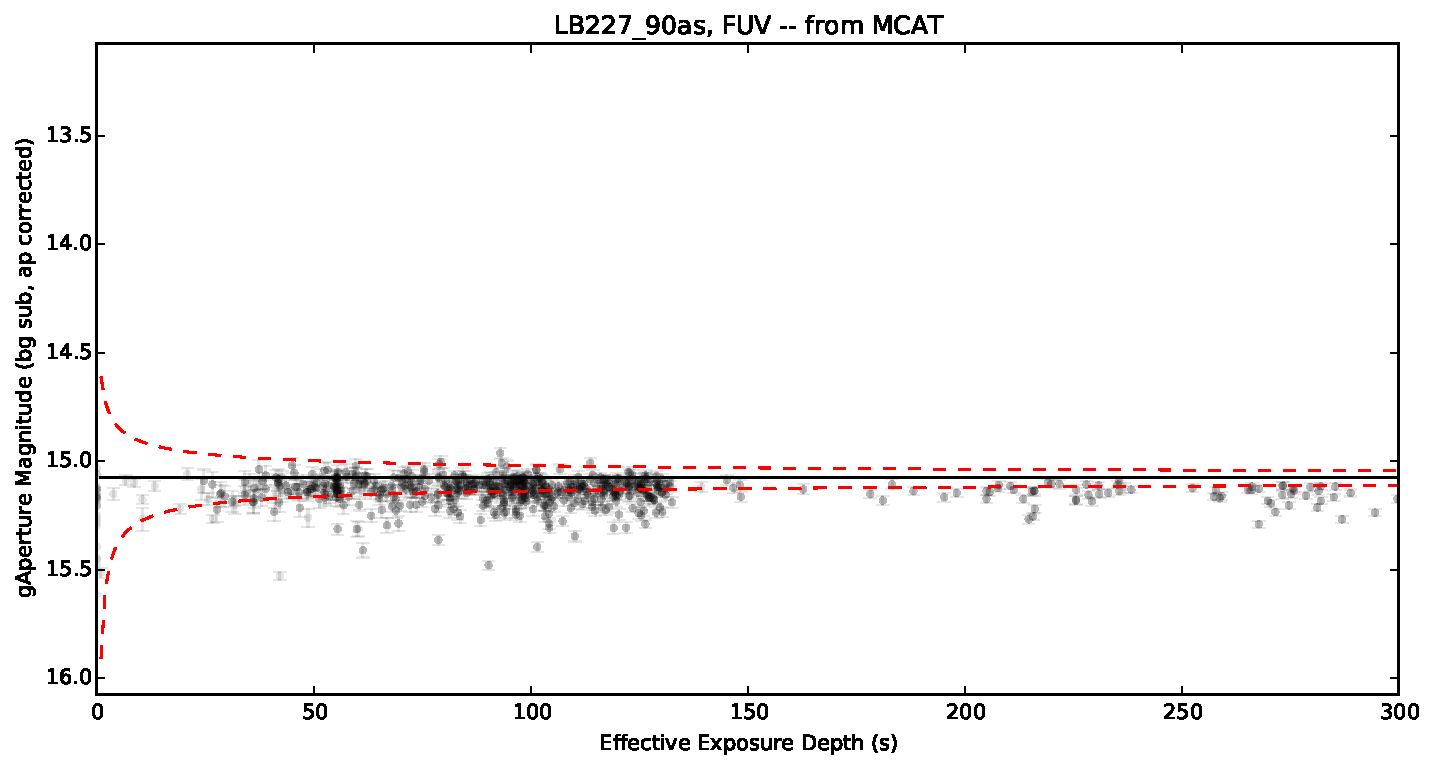
\includegraphics[scale=0.35]{LB227_90as_ABMag_FUV_MCAT.pdf}
\caption{Comparison of gPhoton FUV fluxes for LB227 to the catalog reference value of 15.076 AB Mag (solid line) as a function of exposure depth. The aperture had a radius of 90 arcseconds and backgrounds estimates were drawn from the visit-level MCAT. The dashed lines denote ideal 3 sigma scatter as predicted from counting statistics. The error bars on the points denote 1 sigma.
\label{ldsabsphotfuvmcat}}
\end{figure}

\begin{figure}
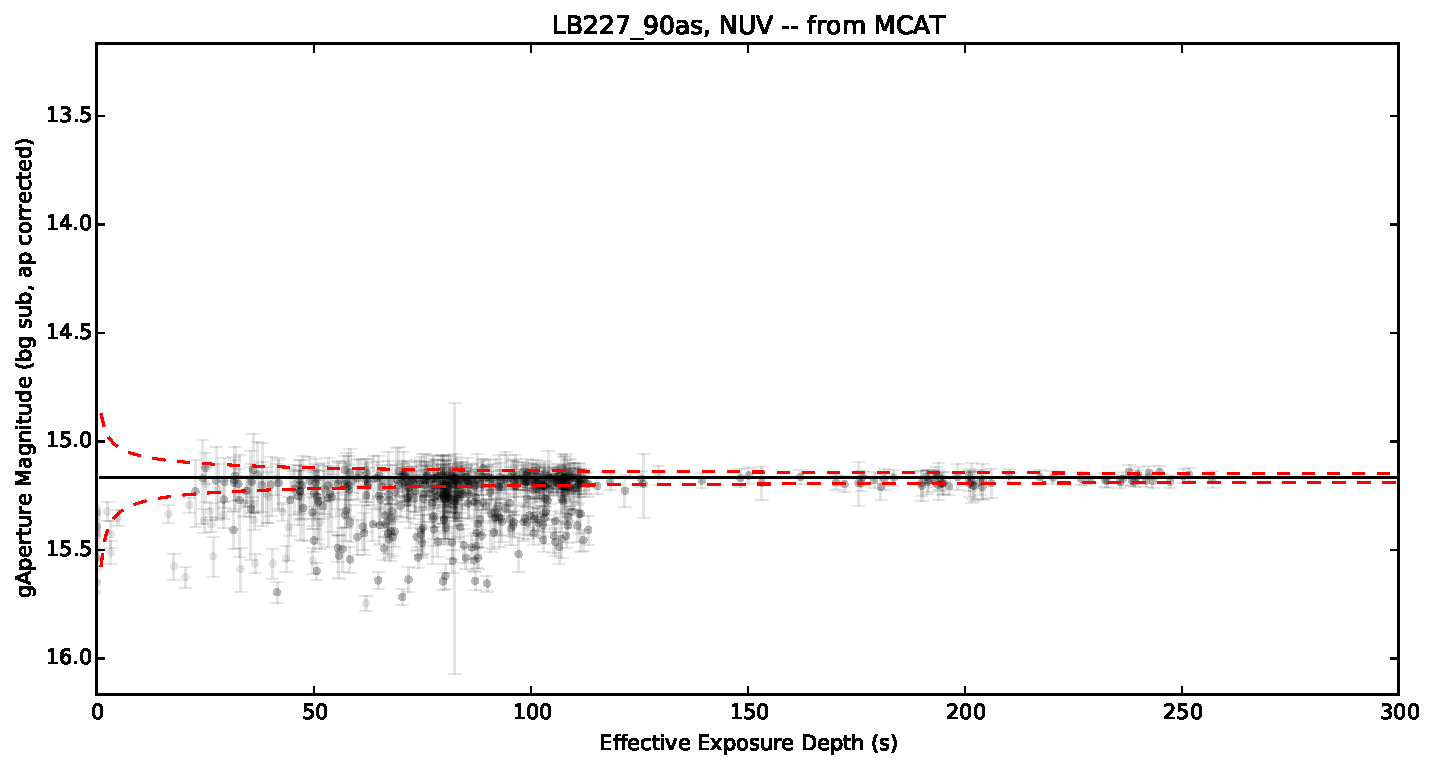
\includegraphics[scale=0.35]{LB227_90as_ABMag_NUV_MCAT.pdf}
\caption{Comparison of gPhoton NUV fluxes for LB227 to the catalog reference value of 15.168 AB Mag (solid line) as a function of exposure depth. The aperture had a radius of 90 arcseconds and background estimates drawn from the visit-level MCAT. The dashed lines denote ideal 3 sigma scatter as predicted from counting statistics. The error bars on the points denote 1 sigma.
\label{ldsabsphotnuvmcat}}
\end{figure}

\section{Example Science Application - Stellar Flares From CR Draconis}
\label{scienceexamples}
CR Draconis (HIP 79796) is a fairly bright ($V \sim 10$) binary star system composed of two M dwarfs located $\sim 20$ pc away in a slightly eccentric orbit with a period of $\sim 4$ years \citep{tam2008}, and has been known to exhibit flares for many decades now \citep{cri1970}.  The system was identified as a high-amplitude variable in the second version of the GALEX Ultraviolet Variability (GUVV-2) Catalog \citep{whe2008}, where a maximum NUV flux difference of two magnitudes was identified within the available visits at that time.  \citet{wel2006} studied one CR Draconis' flare events with high temporal sampling by extracting light curves from sky-projected, ``extended'' (-x) photon list files, produced as non-standard products of the GALEX mission pipeline.

Using our gPhoton pipeline, we have searched for flares from the CR Dra system using all available GALEX data. The largest observed flare in GALEX is the one reported in \citet{wel2006}, but we also see seven additional flares, spanning from 2003 through 2011 (nearly 2 full orbits of the binary).  Fig.\ \ref{crdraflares} shows each of the identified flares.  When available, the FUV version of the light curves are shown in blue.  Several of the flares are double-peaked, and some show elevated levels of flux before or after the flare event.  There is also a range of amplitudes and durations, with some increasing in flux by less than a factor of two and lasting only a few minutes in duration.  These short-duration flares have less an energy than the longer duration, stronger flares, but also can occur more frequently, and thus may still impact the habitability of exoplanets in those systems \citep[e.g.,][]{ram2013}.  While the total energy in a given flare event would be lower, there is also an increased chance for flare-planet alignment.  There have also been studies of the flare rates in resolved M dwarf binaries as a function of orbital separation.  The number of such binaries is small, but CR Draconis is one candidate, and given that the GALEX time baseline extends two full orbital periods, could improve the statistics from previous studies \citep{tam2008}.  {\color{red}Is the difference in flare times for FUV and NUV real, or a bug in the code, or an effect of using $t_{\rm{mean}}$ that may result in different time stamps per point.  Should only differ by a few seconds though, so seems unlikely it would show up that clearly.}

\begin{figure}
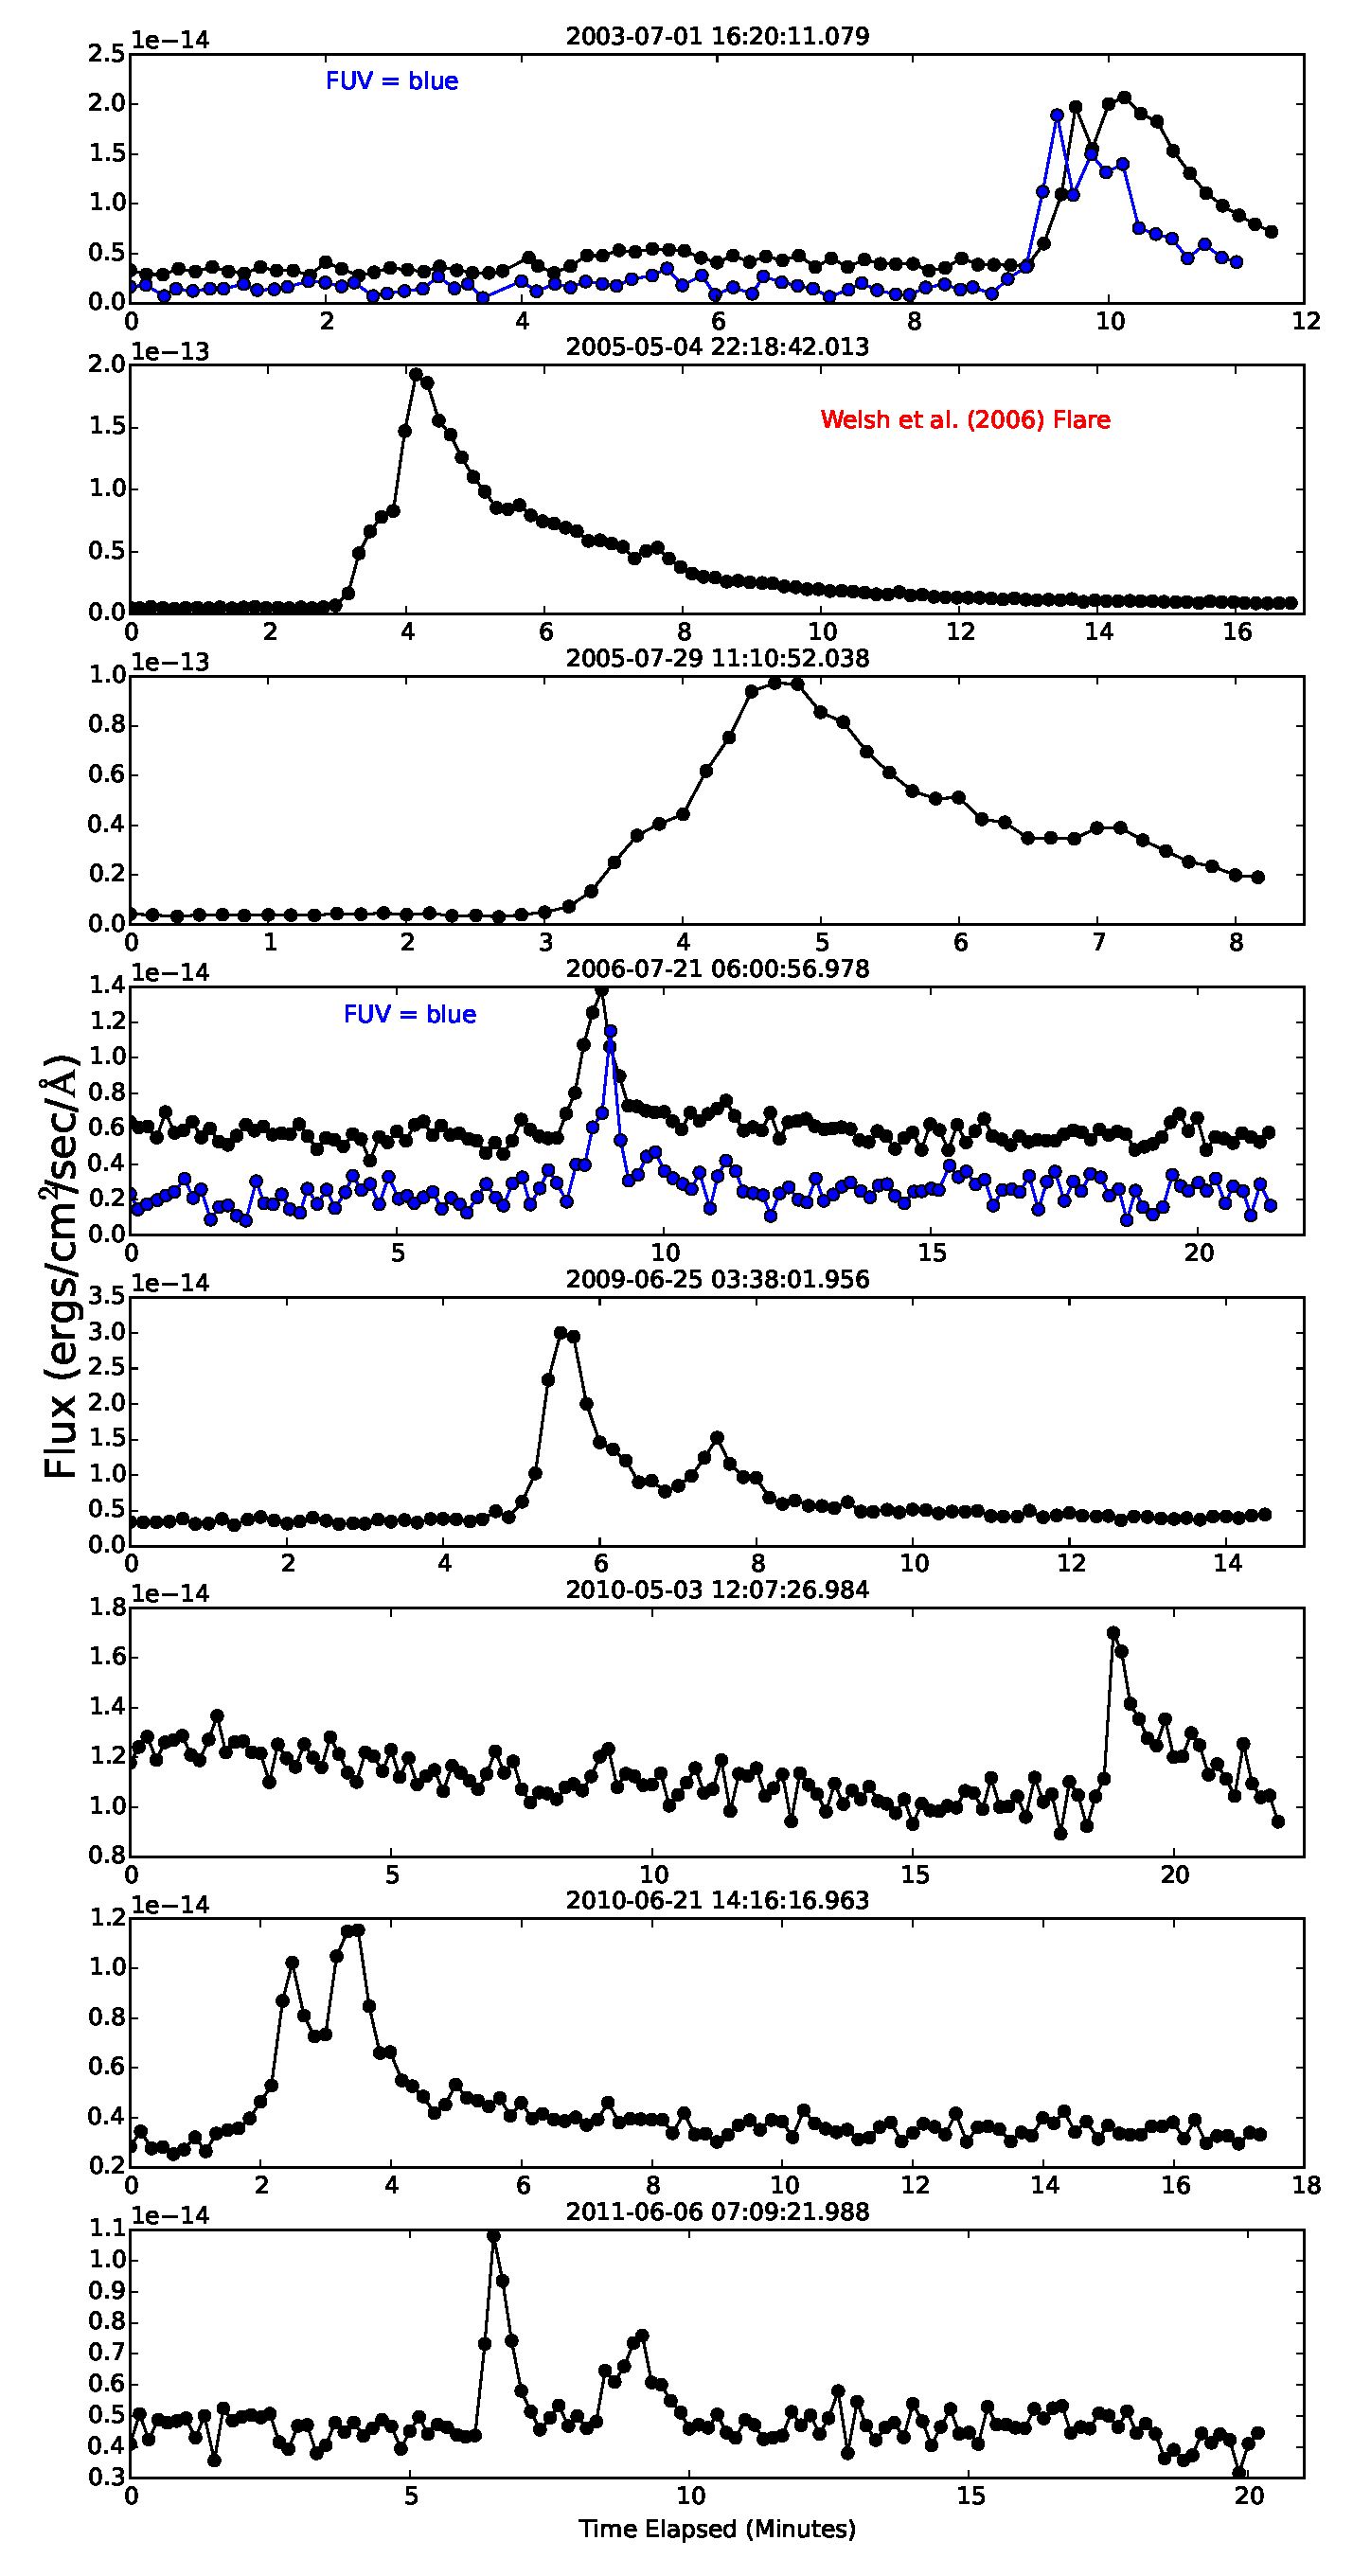
\includegraphics[scale=0.375]{FigCRDraFlares.eps}
\caption{Flares detected on CR Draconis using gPhoton, across the lifetime of the mission.  When available, FUV light curves are plotted (in blue) along with the NUV curves (in black).  Fluxes have not been aperture corrected. \label{crdraflares}}
\end{figure}

A detailed analysis of the flares is beyond the scope of this introductory paper, which serves to present the software itself, and is reserved for future papers that will focus on the astrophysics of flare stars with gPhoton.  However, it is instructive to provide some short scripts demonstrating the basic work flow when creating the plot shown here.  To define our photometric aperture, we used gMap to construct a deep coadd image, centered on CR Draconis, using all available photon events (Fig.\ \ref{crdracoadd}).  Here's the example script that was used, which assumes you have installed gPhoton such that the software lies in your PYTHONPATH environment variable, and thus can be imported as a package (see Inline Supplementary Code \#1, available in the online version of the article):

%InlineCodeSupplementary01.txt gets placed here in the online version of the article.

With our apertures defined (we also adjusted the center of the apertures, due to the moderate proper motion of the star), we can construct our light curve file using gAperture.  Here's the example script that was used to create the CSV file (see Inline Supplementary Code \#2, available in the online version of the article):

%InlineCodeSupplementary02.txt gets placed here in the online version of the article.

After the CSV file is created, we wrote a separate script that reads in the CSV file, converts the $t_{\rm{mean}}$ timestamps from GALEX time to Julian Date, and then defined x-axis boundaries to center on each of the eight flare events of interest.  Note that we did not apply aperture corrections to the fluxes shown in Fig. \ref{crdraflares}, but such corrections are available in Fig.\ 4 in \citet{mor2007}.  A simple interpolation scheme is provided in gPhoton, using those values, called ``apcorrect1'' within the ``galextools.py'' module.

\begin{figure}
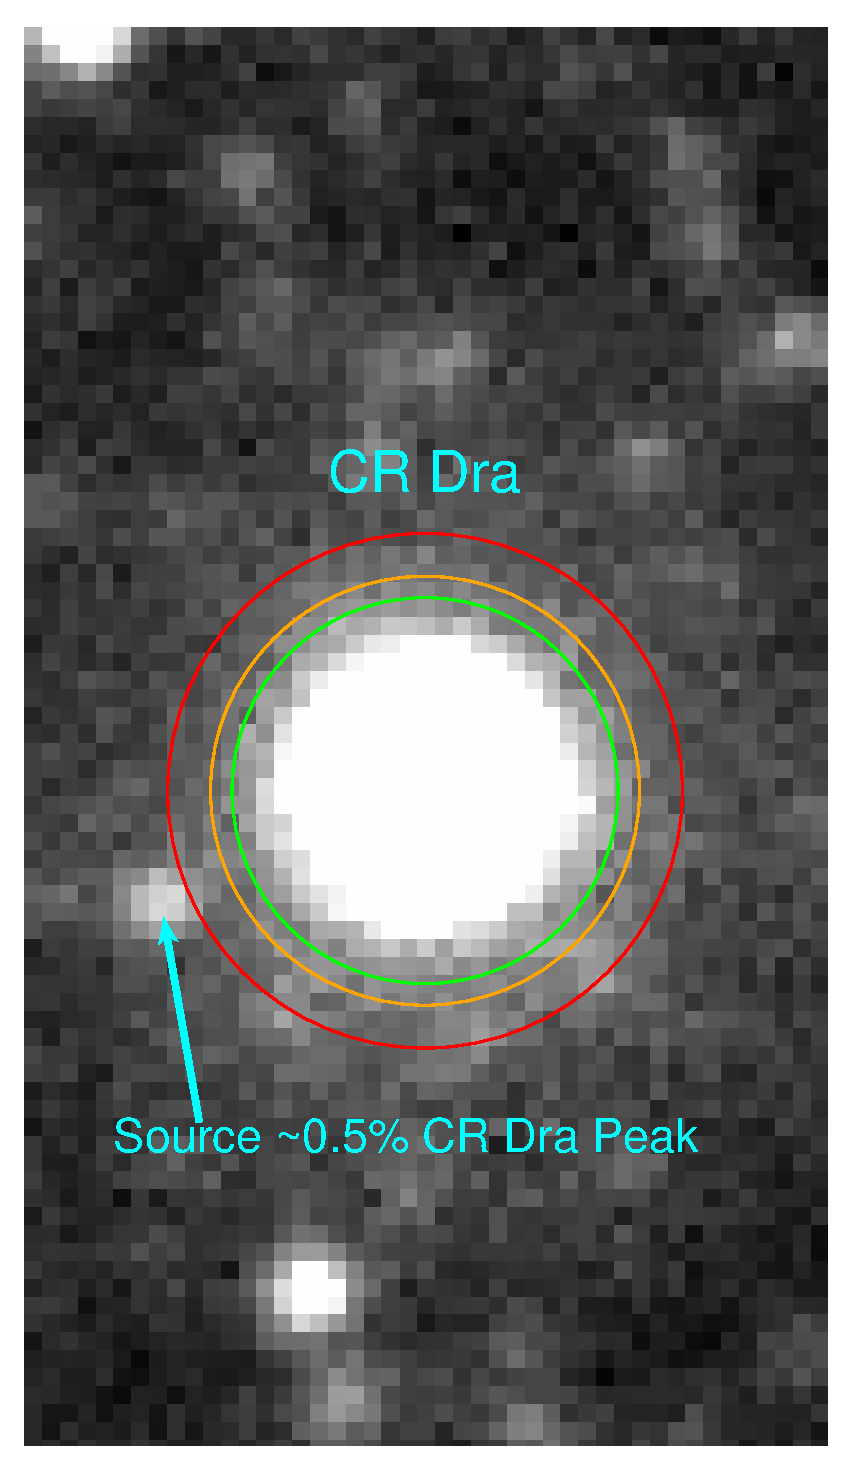
\includegraphics[scale=0.375]{FigCRDraCoadd.eps}
\caption{Deep coadd image of CR Draconis using all available NUV photon events.  The image is in counts, since we are only looking to define our photometric aperture and search for possible contamination sources.  The aperture, inner annulus, and outer annulus for photometry are represented by the green, orange, and red circles, respectively.  There is a source to the lower left that is $\sim 0.5$\% the peak of CR Draconis itself.  Although testing showed it did not have a major impact on the photometry significantly, we still define our apertures such that it is not included within them.\label{crdracoadd}}
\end{figure}


\section{Conclusion}

The GALEX mission has already proven to be extremely productive, and is likely to be one of the most influential ultraviolet astronomical surveys for the foreseeable future.  Nevertheless, even when preparation of the higher level data is well documented and understood by future researchers, the priorities or interests of those users may not be the same as the data creators or archivists. In such cases, their normal recourse would be to go back to some minimally reduced version of the data and create their own procedure for further reducing the data. This can be onerous, time consuming, or impossible depending on the type of data, the quality of the documentation, and the availability of original team members to answer inevitable questions. The burgeoning practice of ``reproducible research'' seeks to address this, to some extent, by making the actual methods (as opposed to mere descriptions of the methods) available to researchers.

The gPhoton project is a trial into a new paradigm for data archiving, where the correlation between minimally reduced and high level data is explicitly laid bare through open-source software.  That machinery is archived for future researchers to make modifications to the reduction methodology with minimal overhead or barriers to entry.  Specific to GALEX, the gPhoton project simplifies, and in some cases enables, analyses using this data that were previously difficult-to-prohibitive, especially those related to short time domain photometry at the intra-visit level.

While the gPhoton project is an effort to calibrate and make available the GALEX photon-level data specifically, some of the techniques described here can be applicable to other observational databases that make use of non-integrating detectors, particularly microchannel plates. The fact that spatial analyses can be performed by making direct queries at the photon-level data, rather than artificially degrading the spatial components of the data by integrating and interpolating onto image maps, offers potential advantages in terms of both the flexibility of the data archive and the computational cost of analysis. The corresponding data management and volume issues associated with storing and retrieving massive amounts of photon-level data is non-trivial, but also entirely solvable with appropriate use of existing database and storage technology. The behavior of the GALEX detector during very short timespans (which correspond to very small spatial sampling of the detector) is not well characterized, and further work on improving the resolution of the detector response, as well as correctly propagating flux uncertainties, will be required to derive the maximum utility from the photon-level data.

\section{Acknowledgments}
{\color{red}Place acknowledgments here, waiting to here back from Rick White about this.  Also need to add, at least, MAST acknowledgment, GALEX one, Simbad one.  Anything else?} We wish to thank the GALEX beta testers for their feedback and patience, particularly Raghvendra Sahai (JPL). We also want to thank several former members of the GALEX mission team including Patrick Morrissey, Ted Wyder, Karl Forster, and Don Neill.

\bibliography{gphoton}

\end{document}
